\documentclass{fast-nuces-bs}
%\documentclass{article}

\usepackage{blindtext}
\usepackage{mathptmx}% Times Roman font
\usepackage[T1]{fontenc}
\usepackage{lipsum} 
\usepackage{sectsty}
\usepackage{tikz-uml}
\usepackage{titlesec}
\usepackage{longtable}
\usepackage{booktabs}
\usepackage{url}
\usetikzlibrary{positioning}

% Information about the Thesis 
% -----------------------------------------------------------------------------
% (All are compulsory, do not delete any line other than author Information)
% For e.g., usually there are 3 students in a group, so leave authorone, 
% authortwo, and authorthree, and delete authorfour.
%%%%%%%%%%%%%%%%%%%%%%%%%%%%%%%%%%%%%%%%%%%%%%%%%%%%%%%%%%%%%%%%%%%%%%%%%%%%%%%
\department{FAST School of Computing}
\faculty{Software Engineering}
\degreeyear{2026}
\degreemonth{October}
\degreename{Software Engineering}
\campuscity{Islamabad}
\authorone{Ahmed Javaid}{22I-2530}
\authortwo{Rafay Ul Haq}{22I-2520}
\authorthree{Soban Ahmad}{22I-2460}
\supervisor{Mr. Irfan Ullah}
% The inherited template session dates are not verified for this team.
\sessionduration{Pending team confirmation}
\cosupervisor{Pending applicability confirmation}
% University Officers page indexed excerpt checked 11 October 2026.
\deanname{Dr. Jawwad Ahmed Shamsi}
% Current official Islamabad leadership directory checked 11 October 2026.
% Names are metadata; no approval or signature is implied.
\directorname{Dr. Waseem Shahzad}
\hodname{Dr. Atif Aftab Ahmed Jilani}
\fypcoordinatorname{Name of FYP Coordinator}
\title{Investify}
% Bridge the report front matter to the official class's existing metadata.
\makeatletter
\newcommand{\projecttitle}{\@title}
\newcommand{\studentone}{\@authoronename{} (\@authoroneroll)}
\newcommand{\studenttwo}{\@authortwoname{} (\@authortworoll)}
\newcommand{\studentthree}{\@authorthreename{} (\@authorthreeroll)}
\makeatother
%%%%%%%%%%%%%%%%%%%%%%%%%%%%%%%%%%%%%%%%%%%%%%%%%%%%%%%%%%%%%%%%%%%%%%%%%%%%%%%

%%%%%%%%%%%%%%%%%%%%%%%%%%%%%%%%%%%%%%%%%%%%%%%%%%%%%%%%%%%%%%%%%%%%%%%%%%%%%%
% Former document starts below this
\begin{document}

%\begin{acknowledgements}
%	Your acknowledgments here
%\end{acknowledgements}

%\begin{abstract}
%Briefly state the (1) research problem, (2) methodology, (3) key results, and (4) conclusion. Generally, abstracts are between 150 and 200 words–roughly 10-15 sentences.
%\end{abstract}

\cleardoublepage
\pagenumbering{roman}
\chapter*{Students' Submission}
\addcontentsline{toc}{chapter}{Students' Submission}
We submit this report for the FYP-1 Mid-Evaluation of \textit{\projecttitle}, Fall 2026, Department of Software Engineering, FAST--NUCES Islamabad. It documents our implemented modules, evaluation results and remaining development plan. We accept responsibility for the submission and its stated contributions.

\vspace{1.5cm}
\begin{tabular}{p{0.53\textwidth}p{0.35\textwidth}}
\studentone & Signature: \rule{0.20\textwidth}{0.4pt}\\[1.2cm]
\studenttwo & Signature: \rule{0.20\textwidth}{0.4pt}\\[1.2cm]
\studentthree & Signature: \rule{0.20\textwidth}{0.4pt}
\end{tabular}
\par\vspace{1cm}\noindent Date: \rule{0.30\textwidth}{0.4pt}

\chapter*{Anti-Plagiarism Statement}
\addcontentsline{toc}{chapter}{Anti-Plagiarism Statement}
We declare that sources, reusable software, pretrained models and external data used in this project are acknowledged and referenced. The report distinguishes our implementation and integration work from external components. Development assistance is disclosed in the tool-use statement in Appendix~\ref{app:handbook}. We accept responsibility for accurate attribution and for the material submitted.

\vspace{1.5cm}
\begin{tabular}{p{0.53\textwidth}p{0.35\textwidth}}
\studentone & Signature: \rule{0.20\textwidth}{0.4pt}\\[1.2cm]
\studenttwo & Signature: \rule{0.20\textwidth}{0.4pt}\\[1.2cm]
\studentthree & Signature: \rule{0.20\textwidth}{0.4pt}
\end{tabular}
\par\vspace{1cm}\noindent Date: \rule{0.30\textwidth}{0.4pt}

\chapter*{Authors' Declaration}
\addcontentsline{toc}{chapter}{Authors' Declaration}
We declare that this report describes the work delivered by the Investify project team for FYP-1 Mid-Evaluation. The member responsibilities and delivered modules are recorded in Chapter~9. Scientific results, limitations and external contributions are identified accurately. Each member accepts responsibility for understanding and defending their contribution and the integrated system.

\vspace{1.5cm}
\begin{tabular}{p{0.53\textwidth}p{0.35\textwidth}}
\studentone & Signature: \rule{0.20\textwidth}{0.4pt}\\[1.2cm]
\studenttwo & Signature: \rule{0.20\textwidth}{0.4pt}\\[1.2cm]
\studentthree & Signature: \rule{0.20\textwidth}{0.4pt}
\end{tabular}
\par\vspace{1cm}\noindent Date: \rule{0.30\textwidth}{0.4pt}

\chapter*{Abstract}
\addcontentsline{toc}{chapter}{Abstract}
Investify is an educational equity decision-support prototype combining technical indicators, financial-news sentiment and explanations checked against model evidence. Its historical pipeline uses exchange-session alignment, causal features and purged chronological evaluation. A verifier checks displayed claims independently of structured payloads and supplies a checked fallback.

An NVDA experiment covers 1,509 price sessions from January 2018 to December 2023 and 6,768 news rows. Clean five-session macro-F1 is 0.2843 versus a random baseline of 0.3287; a deliberate future-looking feature triggers the leakage control. Independent isotonic calibration produces only Buy decisions. A multiclass temperature revision preserves the raw Buy/Hold/Sell distribution but exposes near-uniform probabilities, so low-confidence cases abstain. Original social classifiers are compared on 24 held-out reference-labelled posts. Risk profiling implements thirteen Grable--Lytton items with capacity constraints and a direction-preserving confidence policy. The live interface demonstrates evidence inspection, profile calculation, explanation rejection and recovery. These results establish implemented controls and traceability; useful prediction, student-model adaptation and participant acceptance remain later evaluation goals.

\chapter*{Acknowledgments}
\addcontentsline{toc}{chapter}{Acknowledgments}
We acknowledge Mr. Irfan Ullah's role as project supervisor and the Department of Software Engineering for the FYP assessment guidance and report template. We also acknowledge the authors of the cited datasets, models and software libraries that support the implementation. Their contributions are identified in the report and references.

\chapter*{Executive Summary}
\addcontentsline{toc}{chapter}{Executive Summary}
Investify addresses two practical problems: historical evaluations may use information unavailable at decision time, and a fluent explanation may misstate the evidence behind a prediction. Our prototype combines a temporal evaluation harness with independently checked explanations. The interface exposes the complete technical/news feature context, validates visible text and structured claims separately, and preserves both a rejected candidate and its checked replacement.

The historical pipeline currently evaluates NVDA over 2018--2023. FNSPID was retained as the original comparison corpus, but its midnight-only timestamps and uneven ticker coverage limited precise session alignment. Alpaca/Benzinga provides the new timestamped news snapshot. The source change, selected price basis, data interval and remaining vendor-vintage limitation are documented. The seven-company product universe remains an integration target rather than a completed claim.

Prediction quality remains weak. The clean five-session walk-forward result is below its random comparator. A deliberately centred indicator produces positive lift, demonstrating that the harness detects a known leakage fault. The original isotonic mappings improve Brier score while forcing every decision to Buy. We diagnosed that mechanism and implemented a new global-temperature calibration experiment without replacing the original records. It preserves varied raw classes but approaches uniform confidence; a confidence gate therefore withholds unsupported directional suggestions. Calibration cannot manufacture predictive information.

The risk layer now uses the thirteen-item Grable--Lytton scoring key alongside five capacity factors. Capacity and tolerance reconcile restrictively. The resulting risk allowance controls the confidence required for a suggestion, not the relative sentiment/technical weight. Increasing allowance cannot turn Buy into Sell or Sell into Buy. The profile questionnaire, uncertainty response and explanation-failure path execute live; model outputs and research studies are recorded.

Ahmed Javaid delivered the temporal-data, leakage and CI/delivery work; Rafay Ul Haq delivered the interface, risk and sentiment work; Soban Ahmad delivered the engine, attribution and explanation-verification work. Responsibilities are equal for this evaluation, and members continue practising their modules and the integrated demonstration. The report includes detailed use cases, requirements grouped by module, acceptance checks, individual test cases, revised design models and a dated engineering plan. Hosted Windows/Ubuntu checks and verified artifact delivery provide reproducibility evidence. Later work addresses broader data integration, improved prediction, language-model adaptation, production serving and participant evaluation.

\tableofcontents
\listoffigures
\listoftables
\chapter*{List of Abbreviations}\addcontentsline{toc}{chapter}{List of Abbreviations}
\begin{longtable}{p{.21\textwidth}p{.68\textwidth}}
FYP & Final Year Project\\ FR / NFR & Functional / non-functional requirement\\
NVDA & NVIDIA stock ticker\\ RSI & Relative Strength Index\\ MACD & Moving Average Convergence/Divergence\\
OBV & On-Balance Volume\\ SMA & Simple Moving Average\\ FNSPID & Financial News and Stock Price Integration Dataset\\
XGBoost & Extreme Gradient Boosting\\ SHAP & SHapley Additive exPlanations\\
PoC & Proof of Concept\\ SRS & Software Requirements Specification\\ JSON & JavaScript Object Notation\\
Brier & Brier probability-error score (a name, not an acronym)\\ CV & Cross-validation\\
LLM & Large Language Model\\ QLoRA & Quantized Low-Rank Adaptation\\ CI/CD & Continuous Integration / Continuous Delivery\\
API & Application Programming Interface\\ DEI & Diversity, Equity and Inclusion\\
\end{longtable}


\cleardoublepage
\pagenumbering{arabic}
\chapter{Introduction and Project Vision}
\section{Project Overview}
Investify (F26-003-Investify) is an educational investment advisory project for retail investors. The planned system combines technical indicators, news and social sentiment, and risk information to present a one-week Buy, Hold, or Sell view with understandable, checkable evidence. The proposal was approved with minor modifications concerning contribution clarity, the language-model role, evaluation, transparency, and domain understanding.

\section{Problem Statement}
A retail investor evaluating a company must interpret historical price indicators and a large volume of news and social commentary. A decision label alone does not explain which signals influenced it, how conflicting evidence was handled, how uncertain it is, or whether an action fits the investor's risk constraints. A fluent explanation can misstate recorded values or attributions, while an evaluation using information unavailable at decision time can overstate model quality.

Investify addresses these issues through a temporally controlled evaluation pipeline and explanations tied to recorded inputs and model attributions. Its outputs are educational and advisory; predictive usefulness must be established against explicit comparators, and the system does not execute transactions.

\section{Problem Context and Motivation}
The baseline contains a historical NVDA experiment using technical indicators and financial-news sentiment. It found no demonstrated predictive signal, and its calibrated evaluation records all select Buy. Explaining those records makes the computation and its limitations inspectable; it does not establish a useful trading signal. Financial-text classification supplies evidence about text tone rather than the truth of a headline or a promised return \cite{finbert_card}.

\section{Project Vision}
The user can inspect a view's evidence, understand its uncertainty and coverage, and ask questions without receiving invented values or unsupported causes. The LLM communicates the recorded decision. A separate claim verifier and deterministic fallback govern supported factual statements.

\section{Project Objectives}
Objectives cover point-in-time alignment, engine/baseline comparison, equity social-model transfer and news/social disagreement, capacity/tolerance reconciliation, verified explanations and user understanding, and a reproducible measured system. Implemented components, measured findings, and planned objectives are reported separately.

\section{Project Scope}
The current spike covers NVDA, historical news, one- and five-session experimental horizons, and cached artifacts. Full scope targets a small equity universe, a one-week user horizon, social sentiment, genuine risk conditioning, and a verified LLM. Price-only continuously traded assets provide a later calendar experiment. Brokerage integration and trading execution are excluded.

\section{Project Modules}
Modules cover ingestion/storage, calendar/as-of alignment, feature/sentiment construction, evaluation/controls, prediction/calibration/attribution, risk profiling, explanations/verification, and interface/deployment. The new increment adds complete evidence context at the explanation/interface boundary.

\section{Stakeholders and User Classes}
The primary user seeks educational analysis. The operator maintains data/runtime health. The supervisor evaluates scope and evidence. Each team member must explain and modify their actual work and disclose external assistance and components.

\section{Success Criteria}
Criteria include causal alignment checks, injected faults, held-out predictive/calibration metrics, explanation measures, interpretation tasks, and runtime/installability checks. Existing explanation targets are numeric fidelity at least 0.98, directional consistency at least 0.95, recall at least 0.80, and unverifiable rate at most 0.15. Planned bounds are not measurements.

\section{Constraints and Assumptions}
The local clone lacks the training store/raw corpora, and fresh upstream changes could not be checked. Candidate social-model comparison, live LLM/student inference and comprehension evaluation remain pending. Six recorded teacher examples demonstrate construction under a bounded contract. The prototype questionnaire affects a separate technical/news comparator; it does not condition the saved XGBoost predictions or implement the proposal's validated risk instrument. Context/verification checks can run without the training stack.

\section{Ethical, Legal and DEI Considerations}
The interface must explain data age, coverage, uncertainty, actual profile effect, and failure states. An AI explanation is not a guaranteed prediction \cite{sec_ai_alert}. Personal data, annotations, and acceptance work require appropriate privacy, licensing, consent, and truthful records. The advisory boundary must remain clear throughout the journey.

\chapter{Research and Existing Solutions}
\label{chap:research}
\section{Research Method / Approach}
We reviewed the approved proposal slides, panel action register, official mid-report template and rubric. We then read primary papers, original model cards and official product descriptions, and checked the saved scientific results and implementation. Product descriptions establish advertised features; they do not establish an independently audited evaluation protocol. The unsubmitted concept document is used as design reference rather than as an approved scope change.
\section{Existing Solutions / Products}
Wealthfront uses a questionnaire to recommend an allocation\cite{wealthfront_product}. PortfolioPilot offers portfolio analysis and personalized recommendations\cite{portfoliopilot_product}. Danelfin exposes technical, fundamental and sentiment subscores\cite{danelfin_product}. Magnifi offers conversational investment research\cite{magnifi_product}. Bloomberg and LSEG Workspace combine professional market data and news\cite{bloomberg_product,lseg_product}. StockTwits and TradingView provide social discussion or market-charting tools\cite{stocktwits_product,tradingview_product}. These products address different user tasks; Investify evaluates an inspectable historical research path rather than trying to replace a terminal or a licensed adviser.

Ruan and Jiang combine FinBERT-enhanced sentiment, XGBoost and SHAP in a published prediction pipeline\cite{ruan_jiang_2025}. This is close technical prior work, so combining these libraries is not itself our contribution. Li et al. identify training-window information leakage in LLM financial agents\cite{profit_mirage_2025}. Zhang et al.'s 2026 preprint changes one decision-time convention at a time and finds that inflation depends on the fault\cite{alpha_disappears_2026}; it is not peer reviewed. These studies motivate controlled timing comparisons and a declared null-result path.
\section{Comparison of Existing Solutions}
\begingroup\small
\begin{longtable}{p{.23\textwidth}p{.12\textwidth}p{.16\textwidth}p{.13\textwidth}p{.12\textwidth}p{.13\textwidth}}
\caption{Comparison on the five proposal criteria.}\label{tab:existing-solutions}\\\toprule Solution & Risk profile & Formal + informal sentiment & Explainable predictions & Leakage-safe evaluation & Verified natural language\\\midrule
Wealthfront & Risk quiz & Not specified & Allocation explanation & Not assessed & Not specified\\
PortfolioPilot & Risk preferences & Not specified as paired features & Portfolio recommendations & Not assessed & Not specified\\
Danelfin & Low-risk score; personal profile not established & Sentiment subscore; register separation unclear & Feature subscores & Not assessed & Not specified\\
Magnifi & Personal help & Not specified & Research chat & Not assessed & Not specified\\
Bloomberg / LSEG & Risk tools & News; other content varies & Analytics and research & Product-dependent; not assessed & Record-level guard not established\\
StockTwits / TradingView & Not established here & Social discussion / charts and news & Signals and charts & User-script dependent & Not established here\\
Published FinBERT + XGBoost + SHAP & Not central & News; no paired social experiment identified & SHAP attributions & Study-specific timing & No independent claim guard identified\\
Manual workflow & User judgement & User-selected sources & User reasoning & User-dependent & No automatic checker\\
Investify Mid-1 & Complete score + gate & News; social evaluated separately & All-feature SHAP context & Tested controls; Gate A partial & Template grammar + checked fallback\\
Investify planned & Same profile design & Integrated divergence ablation & SHAP + LLM prose & Broader timing/parity validation & Constrained claims, Mid-2\\
\bottomrule\end{longtable}
\endgroup
``Not specified'' means the inspected public source did not establish that criterion, not that the product lacks it. The manual row describes the workflow targeted by this project, not a measured user-study baseline.
\section{Limitations and Gaps}
The relevant gap is the combination of time-aware evaluation and a checkable explanation. Showing an indicator, a proprietary score or fluent prose does not by itself show that the inputs were available at decision time or that each explanation claim matches the computation. Conversely, checking a claim does not establish a useful predictor. The current project limitations are consolidated in Section~\ref{sec:limitations}.
\section{Proposed Solution}
The learner receives the model's probabilities, full evidence and a separate risk-policy outcome. A deterministic verifier checks known claims and retains the reason for rejection before emitting a checked replacement. The planned LLM translates the same record into accessible prose. Its design and evaluation are in Section~\ref{sec:llm-design}.
\subsection{Contribution and Evaluation}
\begin{enumerate}
\item \textbf{C1: Leakage-audited point-in-time harness with a permanent canary.} Implemented timing, scaling and label-end checks; evaluated by unit tests and fixed leakage arms. The centred Bollinger fault fires. Broader historical availability and the full proposal Gate A remain partial.
\item \textbf{C2: Deterministic claim verifier with retained rejection and checked fallback.} Implemented for the template grammar; evaluated using independent prose/JSON corruptions, omission tests and the live recovery path. Free-prose extraction is a Mid-2 deliverable.
\item \textbf{C3: Cross-register divergence features with a pre-registered ablation.} Planned. Evaluate a news-only model against news/social and divergence variants using shared chronological folds and settings, with the protocol fixed before running the comparison.
\end{enumerate}
As stated on proposal slide 8, no novelty is claimed in sentiment scoring, gradient boosting, SHAP-to-text or QLoRA, and no profit claim is made. The contributions concern controls and their evaluation, not the mere use of these components.
\section{Complex Computing Problem}
The requirement is to justify a stock-research outcome using observations that arrive on different clocks, preserve the information available at decision time, reconcile capacity with tolerance and keep every displayed claim consistent with the underlying computation. These requirements conflict when a fluent explanation or a personalized response would otherwise hide weak evidence.
\begin{longtable}{p{.26\textwidth}p{.63\textwidth}}
\caption{Seoul Accord characteristics applied to the project.}\label{tab:ccp}\\\toprule Characteristic & Project evidence and boundary\\\midrule
Conflicting requirements & Readability versus checkability; capacity versus tolerance; personalization versus privacy\\
No obvious solution & Timing and vendor revisions require an explicit information-availability model, not just a random train/test split\\
Depth of knowledge & Label overlap, calibration, attribution and claim verification require different mathematical models\\
Unfamiliar issues & Retroactive price adjustment, early closes and revised publication times create silent evaluation faults\\
Beyond routine practice & Team-built fault controls and record-based rejection tests complement libraries\\
Diverse stakeholders & Learner, operator and supervisor have different criteria, but the current operating roles are modest\\
Significant consequences & Unfounded certainty may mislead a non-expert interpreting a stock signal\\
Interdependence & Store, feature construction and evaluation are coupled; much of the pipeline is still sequential\\
Ill-defined requirements & Whether short-horizon predictive information exists must be discovered rather than assumed\\
\bottomrule\end{longtable}
This is a requirement-level argument adapted from concept Section 5. It does not treat every characteristic as equally strong.
\section{Technical Challenges}
The main challenges are timestamp precision, available-label boundaries, calibration collapse, social-domain transfer and consistent text/JSON claims. XGBoost\cite{xgboost_2016} and SHAP\cite{shap_2017,treeshap_paper} supply algorithms; the project must control how their inputs, outputs and claims are evaluated. Purged evaluation is motivated by overlapping financial labels\cite{deprado_2018}.
\section{Research Findings and Design Decisions}
The FNSPID precision audit led to a separate timestamped Alpaca/Benzinga experiment. Isotonic calibration collapsed the final classes; the subsequent bounded temperature fit produced near-uniform probabilities and motivated abstention. The full profile is used as a confidence gate rather than changing model direction. The social study motivates evaluating equity transfer before adding divergence. The current template verifier precedes any prompted LLM or QLoRA work\cite{qlora_2023,phi3_2024}.
\section*{Stock Market Background and Design Implications}
\addcontentsline{toc}{section}{Stock Market Background and Design Implications}
\label{sec:market-background}
\subsection*{Price Formation, Liquidity and Trading Sessions}
A share represents an ownership interest in a company. Secondary-market prices arise when buyers and sellers transact through trading venues. A bid is an offered buying price and an ask is an offered selling price; their difference is the spread. Market orders seek execution at available prices, while limit orders restrict the acceptable price. A daily close summarizes completed trading and is not a guarantee that a later order can be filled at that price\cite{sec_orders,sec_execution,sec_participants}. A model trained on daily bars cannot infer an intraday order book or assume unlimited liquidity.

Trading takes place on a calendar. US equity sessions contain holidays and early closes; five trading sessions can span more than five calendar days\cite{nyse_calendar}. An announcement after the close belongs to a different information set from one received before it. Our labels use observed price-session endpoints. The inherited fixed 16:00 New York news cutoff is recorded, including its early-close limitation.

\textbf{Design implication:} use an exchange calendar, preserve event and acquisition times and join completed news sessions backward to prices. Evaluate execution assumptions separately before any future trading claim. The present UI reports a historical date and horizon and has no order-execution path.
\subsection*{Price Drivers and the Short-Horizon Noise Problem}
Earnings and guidance can change expectations of future cash flows; valuation also depends on the return investors demand. Monetary policy and interest rates can affect discount rates, financing costs and alternatives to equities. Sector and index movements, institutional flows and liquidity can move a stock alongside its own news. These are reasons to avoid explaining a price change from a single headline. The project's eleven inputs contain price/volume summaries and headline sentiment; they are not a complete valuation or macroeconomic model.

Market efficiency treats prices as responding to available information\cite{fama_1970}. It does not prove that every market is always efficient or that no prediction can work. It does explain why widely observed short-horizon signals can have little remaining advantage once information, costs and timing are handled correctly. Positive historical performance requires a meaningful comparator and an out-of-sample protocol.

\textbf{Design implication:} compare with stratified-random and linear baselines, preserve weak findings and keep SHAP statements about model use separate from economic causation. A probability is a class estimate, not an expected return. The current no-signal result is a reason to abstain rather than to claim market insight.
\subsection*{The Five Technical Inputs}
Let $P_t$ be the completed closing price, $V_t$ traded share volume, and $\Delta P_t=P_t-P_{t-1}$. All windows below end at $t$; no centred window is allowed in the clean features. Indicator guides describe their usual interpretation\cite{fidelity_rsi,fidelity_macd,fidelity_obv}; the exact implemented formulas are in \nolinkurl{features/indicators.py}.
\begin{description}
\item[RSI(14)] With $g_t=\max(\Delta P_t,0)$ and $\ell_t=\max(-\Delta P_t,0)$, the implementation uses simple fourteen-session averages: $RS=\overline g_{14}/\overline\ell_{14}$ and $RSI=100-100/(1+RS)$. Completed all-gain/all-loss windows yield 100/0; a completed flat window yields 50. Warm-up remains missing.
\item[MACD histogram] $M_t=EMA_{12}(P)_t-EMA_{26}(P)_t$ and $H_t=M_t-EMA_9(M)_t$, where $EMA$ uses $\alpha=2/(n+1)$. This measures components of price momentum; its sign does not prescribe a trade.
\item[Distance from SMA200] $D_t=(P_t-SMA_{200,t})/SMA_{200,t}$. The long window means early rows do not have a complete value.
\item[Bollinger position] $B_t=(P_t-L_t)/(U_t-L_t)$, with $L_t=\overline P_{20}-2s_{20}$ and $U_t=\overline P_{20}+2s_{20}$. The sample standard deviation describes trailing variability. Values can lie outside $[0,1]$; a zero-width band is missing.
\item[OBV slope] $OBV_t=OBV_{t-1}+\operatorname{sign}(\Delta P_t)V_t$ and $O_t=(OBV_t-OBV_{t-14})/14$. This is a price-associated volume summary, not an observation of investors' intentions.
\end{description}
\textbf{Design implication:} expose the maintained definition and actual recorded value beside its SHAP effect. A value's sign and its attribution sign answer different questions. Direct perturbation checks verify that changing a future price cannot change an earlier clean feature.
\subsection*{The Six News Inputs, Absorption and Manipulation}
FinBERT assigns positive, neutral and negative headline probabilities\cite{finbert_paper,finbert_card}. For headline $i$, polarity is $q_i=p_i^{+}-p_i^{-}$. Let $n_t$ be the scored-headline count and $a_t$ the contributing session's average polarity. The implemented six news features are:
\begin{align*}
\text{mean\_polarity}_t &= a_t=\frac{1}{n_t}\sum_{i=1}^{n_t}q_i, & \text{mention\_volume}_t &= n_t,\\
\text{mom\_3d}_t &= \overline a_{3,t}-a_{t-3}, & \text{mom\_7d}_t &= \overline a_{7,t}-a_{t-7},\\
\text{volume\_z}_t &= \frac{n_t-\overline n_{20,t}}{s_{n,20,t}}, & \text{dispersion}_t &= s_{a,5,t}.
\end{align*}
Momentum allows shorter initial rolling windows but still needs the shifted prior value. Attention z-score needs at least five observations and a nonzero standard deviation; dispersion needs at least two. Dispersion is variation in session-average tone, not disagreement between individual headlines. Headline count is news attention, not traded share volume.

News can be anticipated, absorbed quickly or overwhelmed by other information. Tone can also reflect rumours, selective reporting or coordinated discussion. Neither a positive headline nor social agreement proves truth or price impact\cite{sec_ai_alert}. The paired social study therefore measures sentiment agreement on its frozen sample rather than investment performance. Cross-register divergence is planned and will be tested with shared evaluation settings.

\textbf{Design implication:} store the later creation/update timestamp for the new news snapshot, disclose coverage and missing features, and use a strict prior-session join. The future explainer must describe conflicting model contributions without inventing absent social values or claiming that a headline caused a return.
\subsection*{Volatility Regimes and Corporate Actions}
The distribution of returns and the usefulness of a signal may change between quiet and volatile periods. The same indicator value need not imply the same future outcome. Calibration fitted on one period may transfer poorly to a later refitted classifier, so mode and period identities remain visible.

Splits change share count and price units. NVIDIA's four-for-one 2021 split and ten-for-one 2024 split are documented by the issuer\cite{nvda_split_2021,nvda_split_2024}. The new historical prices use a current-vintage SIP split adjustment, including the vendor's action vintage, without cash-dividend adjustment. A discontinuity in raw prices must not be mistaken for an economic return; adjusted close and total return are different conventions.

\textbf{Design implication:} pin adjustment policy and data vintage, preserve issuer-action references and assess regimes and dividend treatment separately. Compare calibration on its declared fit/evaluation periods. The present model's uniform-confidence outcome supports no directional recommendation across either example profile.

\section*{Model Inventory and Adaptation}
\addcontentsline{toc}{section}{Model Inventory and Adaptation}
\label{sec:model-inventory}
\begingroup\small
\begin{longtable}{p{.23\textwidth}p{.29\textwidth}p{.37\textwidth}}
\caption{Checkpoints, tasks, choices, adaptation, licenses and status.}\label{tab:model-inventory}\\\toprule Model/checkpoint & Task, domain and inputs/outputs & Choice, adaptation, license and status\\\midrule
\nolinkurl{ProsusAI/finbert} & Financial headlines to positive/neutral/negative probabilities; polarity is positive minus negative & Chosen for financial text. Original weights, no project fine-tune. News inference completed. Current publisher weights card states CC BY-NC-SA 4.0; pinned-source license context retained.\\
\nolinkurl{ElKulako/cryptobert} & Crypto-social text to three-class sentiment; equity transfer evaluated & Original checkpoint, no project adaptation. MIT model card. Executed on frozen 24-post MSFT held-out set; macro-F1 0.2564.\\
\nolinkurl{cardiffnlp/twitter-roberta-base-sentiment-latest} & Twitter text to three-class sentiment & Alternative social domain. No project adaptation. CC BY 4.0 model card. Same 24 posts; macro-F1 0.6016.\\
XGBoost project model & Eleven price/news features to Buy/Hold/Sell scores and probabilities & Trained by the project; chronological validation. XGBoost software Apache 2.0. Retained frozen/refit model hashes in scientific receipts.\\
OpenAI GPT-6 assistant teacher & Saved record/context to controlled prose; six pilot examples & Teacher name comes from frozen plan. Exact serving revision unavailable. Proprietary service terms. JSON targets assembled deterministically; student not trained.\\
Microsoft Phi-3-mini & Planned local record/context-to-prose student & Original publisher family; exact project checkpoint not selected. MIT publisher model card. Prompted baseline Mid-2; QLoRA Iteration 4\cite{phi3_2024,qlora_2023}.\\
Mistral & Planned fallback local explainer & Exact fallback checkpoint unselected; Mistral-7B-Instruct-v0.3 is an Apache 2.0 publisher candidate. No executed fallback study.\\
\bottomrule\end{longtable}
\endgroup
The executed revisions are \nolinkurl{0bc2ac10dda6929bcb1f77ccc43c7ec5c424f031} (FinBERT), \nolinkurl{9e37c910fe87727cb842a9ac55c6388256fe0f15} (CryptoBERT), and \nolinkurl{3216a57f2a0d9c45a2e6c20157c20c49fb4bf9c7} (Cardiff). These are read from the research reference and paired study receipt. Model cards describe domain and licenses\cite{cryptobert_card,twitter_sentiment_card,phi3_card,mistral_card}; licenses are not inferred from the library used to load a model.


\chapter{Proposal Feedback and Iteration Plan}
\section{Proposal Feedback Summary}
The panel approved the project with minor modifications. PF-01--PF-09 organize the supplied comments into contribution, LLM role, evidence explanation, problem statement, models, metrics, PoC, transparency and market background. The approved slides provide the proposal claims; the unsubmitted concept supplies additional reference design. Status below describes the technical response, not a supervisor closure decision.
\section{Proposal Action Register}
\label{sec:actions}\label{app:actions}
\begingroup\small
\begin{longtable}{p{.07\textwidth}p{.16\textwidth}p{.35\textwidth}p{.10\textwidth}p{.18\textwidth}}
\caption{Panel feedback, action, status and evidence.}\label{tab:panel-actions}\\\toprule No. & Feedback & Action Taken & Status & Evidence\\\midrule
PF-01 & Clear contribution & C1 harness, C2 verifier and planned C3 divergence separated from library inputs & Partial & Section 2.5; leakage results in 6.7\\
PF-02 & Explain LLM benefit & Inputs/outputs, permitted claims, worked example and comparison plan specified & Partial & Section~\ref{sec:llm-design}; prompted evaluation Mid-2\\
PF-03 & Explain technical and sentiment signals & All eleven values/definitions and contributions; conflicts and missing social data explained & Partial & Section~\ref{sec:market-background}; \nolinkurl{test_mideval_context.py}\\
PF-04 & Refine problem & Retail workflow, confidence, records, leakage and unchecked fluent text described & Closed & Section 1.2\\
PF-05 & Model clarity & Executed revisions, tasks, domains, adaptation and licenses listed & Closed & Table~\ref{tab:model-inventory}; frozen study receipts\\
PF-06 & Metrics & Definitions, thresholds and measured/planned populations separated & Partial & Table~\ref{tab:metrics-matrix}; broader evaluation pending\\
PF-07 & Improve PoC & Full profile, independent checks, supported corruptions and checked recovery demonstrated & Closed & Section 6.9; \nolinkurl{test_mideval_policy_explanation.py}\\
PF-08 & Transparency & Onboarding, per-step status/date/confidence/limits and Observe headline requirements added & Partial & MID-FR-21--23; presenter tests; user comprehension pending\\
PF-09 & Market understanding & Price formation, drivers, eleven formulas, absorption, regimes and actions connected to design & Closed & Section~\ref{sec:market-background}\\
\bottomrule\end{longtable}\endgroup
``Closed'' indicates that the requested document/software response is present. PF-01--03 remain partial because divergence, prompted free prose and user benefit are still planned. Appendix A identifies the preserved original feedback.
\section{Iteration Strategy}
Each iteration delivers runnable modules and tests with a separately identified result set. Iteration 1 establishes the data/harness/viewer baseline; Iteration 2 extends engine and services; Iteration 3 adds prompted explanations and measured operations; Iteration 4 compares the adapted student. Weak prediction is a reportable outcome under the proposal gates.
\section{Iteration 1 Plan}
The reference plan calls for hardened ingestion, two-calendar mapping, technical indicators, news features, social selection, an end-to-end linear baseline, a green leakage suite with a firing mutation test, a thin one-company Streamlit view and baselined requirements/design. Table~\ref{tab:proposal-delivered} records the actual outcome of each item.
\section{Iteration 2 Plan}
Extend multi-company data, evaluate XGBoost/calibration/SHAP against the baseline, preregister the divergence ablation, integrate the service and attempt deployment. The engine and deterministic verifier were built early, while usable prediction, integrated divergence and hosting remain open.
\section{Work Breakdown and Responsibilities}
\label{sec:planned-work-division}
Ahmed owns temporal data, the leakage harness and CI/delivery; Rafay owns the interface, profile and sentiment path; Soban owns the decision engine, calibration, attribution and verifier/student work. The user confirmed equal delivered contributions. Chapter 8 records delivery and continuing responsibility.
\begin{longtable}{p{0.21\textwidth}p{0.48\textwidth}p{0.21\textwidth}}\toprule
Member & Proposal-assigned responsibilities & Completion evidence\\\midrule
Ahmed Javaid & point-in-time harness; leakage tests; dual-timestamp schema; parity test; deployment & Actual member work and defence to be recorded.\\
Rafay Ul Haq & risk profiling; sentiment pipeline; degraded operation; acceptance testing; frontend & Actual member work and defence to be recorded.\\
Soban Ahmad & decision engine; Calibration; SHAP; Verifier; QLoRA distillation & Actual member work and defence to be recorded.\\
\bottomrule\end{longtable}

\section{Progress Against Plan}
\begingroup\small
\begin{longtable}{p{.25\textwidth}p{.30\textwidth}p{.34\textwidth}}
\caption{Proposal versus delivered Iteration 1 and recorded deviations.}\label{tab:proposal-delivered}\\\toprule Reference item & Delivered status & Deviation / reason\\\midrule
Hardened ingestion & Timestamp/dedup/store code and versioned inputs & Current-vintage vendor availability is not historically proven\\
Two-calendar mapping & Equity/continuous calendar code and tests & Scientific execution is NVDA only; no crypto generalization study\\
Technical indicators & Five causal indicators & Centred variants exist only as labelled faults\\
News sentiment features & Six FinBERT headline aggregates & FNSPID/yfinance path replaced for new study by Alpaca/Benzinga/SIP because of timestamp gaps and acquisition recovery\\
Social selection study & Two original classifiers executed on 24 held-out MSFT posts & AI reference labels replace the proposed hand-labelled sample; independent human agreement absent\\
Linear baseline end to end & Recorded training/CV/final linear results & UI focuses on saved XGBoost cases; linear result is documented comparison\\
Leakage suite and mutation & Timing tests and centred Bollinger canary & Gate A partial: five-session clean result is below chance, not literal chance-level closure\\
Thin Streamlit slice & Five-step historical evidence/profile/checking flow & Expanded beyond original baseline verdict/status slice\\
Requirements/design baseline & Numbered acceptance and design documents & Formal supervisor approval is not recorded\\
Asset coverage & NVDA model study; separate MSFT social benchmark & Seven equities in approved slides remain future coverage\\
Calibration & Isotonic failure retained; temperature diagnostic added & Temperature reaches its bound and gives no usable confidence signal\\
Risk as model inputs & Full capacity/tolerance calculation and post-hoc gate & Risk is not a classifier feature; $\lambda=2.25$ from concept was dropped because no loss-aversion utility model is implemented\\
Teacher construction & Six OpenAI GPT-6 assistant prose examples, deterministic JSON targets & Concept open-weight teacher replaced by recorded assistant session; prompted student and adaptation unexecuted\\
\bottomrule\end{longtable}\endgroup
\section{Delays, Deviations and Recovery Plan}
Timestamp precision, acquisition/runtime recovery, weak clean prediction and calibration collapse caused deviations. Recovery keeps old results, creates separate experiments and prevents a misleading recommendation. Gate A and Gate B outcomes are stated in Section~\ref{sec:gates}; broader modelling should proceed only with the unmet gate conditions addressed and the null result retained.
\begin{longtable}{p{.18\textwidth}p{.48\textwidth}p{.23\textwidth}}
\caption{Reference iteration milestones and current work.}\label{tab:engineering-dates}\\\toprule Relative checkpoint & Planned deliverable & Owner\\\midrule
Mid-1, week 7 / rubric around week 8 & Data/harness, thin UI and this report & All three\\
Final-1, week 12 & Engine/service and divergence evaluation & Ahmed, Rafay, Soban\\
Mid-2, week 18 & Prompted explainer, constrained claims, NFRs/parity and acceptance preparation & Soban, Rafay\\
Final-2, week 24 & QLoRA comparison, external installation and participant evaluation & All three\\
\bottomrule\end{longtable}
These are proposal-relative milestones, not invented calendar appointments.

\chapter{Software Requirements}
\section{User Interactions}
The learner selects a historical case, inspects evidence, completes a risk profile and checks an explanation. The operator installs the viewer and inspects input failures. Research views expose source-bound studies. The current workflow is historical and educational; the final conversational service remains later scope.
\section{Use Case Diagram}
Figure~\ref{fig:usecases} uses actors outside the system boundary, oval use cases and labelled include/extend relationships. Study preparation is an operator task, not an unimplemented student actor.
\begin{figure}[htbp]\centering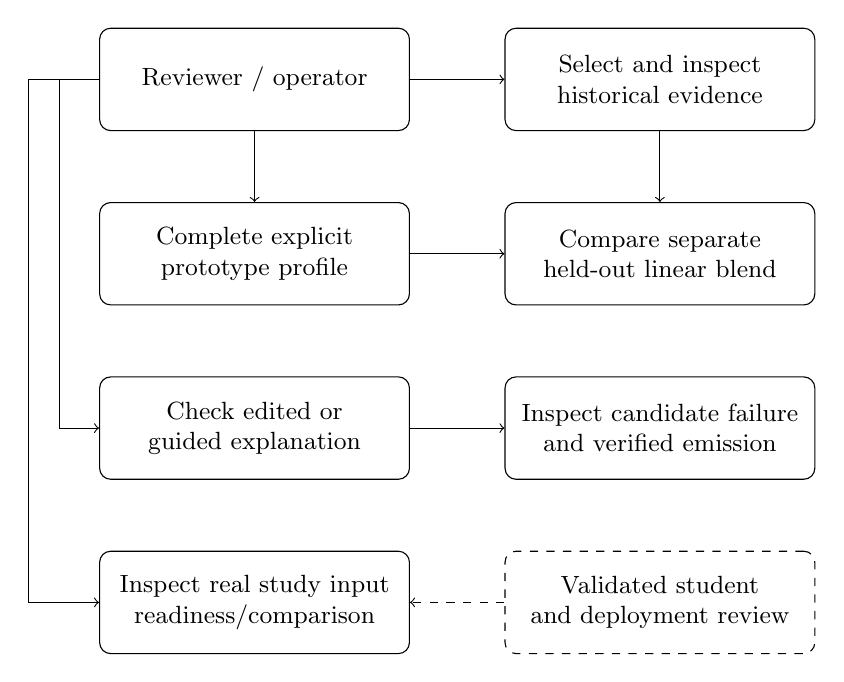
\begin{tikzpicture}[
box/.style={draw,rounded corners,align=center,text width=37mm,minimum height=13mm,font=\small},
pending/.style={box,dashed},node distance=9mm and 12mm]
\node[box] (actor) {Reviewer / operator};
\node[box,right=of actor] (record) {Select and inspect\\historical evidence};
\node[box,below=of actor] (profile) {Complete explicit\\prototype profile};
\node[box,right=of profile] (blend) {Compare separate\\held-out linear blend};
\node[box,below=of profile] (verify) {Check edited or\\guided explanation};
\node[box,right=of verify] (result) {Inspect candidate failure\\and verified emission};
\node[box,below=of verify] (study) {Inspect real study input\\readiness/comparison};
\node[pending,right=of study] (inputs) {Validated student\\and deployment review};
\draw[->] (actor) -- (record);
\draw[->] (actor) -- (profile);
\draw[->] (profile) -- (blend);
\draw[->] (record) -- (blend);
\draw[->] (verify) -- (result);
\draw[->] (actor.west) -- ++(-5mm,0) |- (verify.west);
\draw[->] (actor.west) -- ++(-9mm,0) |- (study.west);
\draw[->,dashed] (inputs) -- (study);
\end{tikzpicture}
\caption{Implemented learner/operator use cases.}\label{fig:usecases}\end{figure}
\section{Detailed Use Cases}
\subsection{UC-01: Select a Historical Decision}
\begin{description}
\item[Actor] Learner.
\item[Precondition] The viewer runs and a registered experiment exists.
\item[Trigger] Select an experiment and session.
\item[Main flow] The loader reads the declared artifact, validates schema and unique sessions, binds its digest and displays class/probabilities for the chosen case.
\item[Exceptions] Missing, malformed or changed evidence produces an error without a substituted decision.
\item[Postcondition] One source/date/digest identifies the active case; an obsolete explanation result is cleared.
\end{description}
\subsection{UC-02: Inspect Technical and News Evidence}
\begin{description}
\item[Actor] Learner.
\item[Precondition] A valid case is selected.
\item[Trigger] Open Evidence and choose a family/feature.
\item[Main flow] Display the recorded value, maintained meaning, raw-score contribution and selected-class direction; expose all eleven inputs in detail.
\item[Exceptions] A missing value remains explicitly missing; an absent social signal is not fabricated.
\item[Postcondition] The learner can trace each displayed feature to the active record.
\end{description}
\subsection{UC-03: Complete the Risk Profile}
\begin{description}
\item[Actor] Learner.
\item[Precondition] Profile form is available.
\item[Trigger] Submit five capacity and thirteen tolerance answers.
\item[Main flow] Validate all choices, sum published tolerance weights, calculate capacity/caps and reconcile the more restrictive tier. Display the binding axis and allowance $R$.
\item[Exceptions] Any unanswered/invalid choice withholds the result. Explicit fictional examples are labelled; Clear removes the profile.
\item[Postcondition] A versioned profile is held only in the local session.
\end{description}
\subsection{UC-04: Apply the Confidence Policy}
\begin{description}
\item[Actor] Learner.
\item[Precondition] Valid case and complete profile.
\item[Trigger] Apply/change the profile or selected case.
\item[Main flow] Calculate $\tau(R)=0.80-0.30R$ and compare the recorded class confidence. Withhold a directional suggestion below the threshold; never reverse its market direction.
\item[Exceptions] Low allowance/confidence produces Observe; an existing Hold signal remains non-directional.
\item[Postcondition] The profile outcome is displayed separately from unchanged model probabilities and SHAP.
\end{description}
\subsection{UC-05: Check an Explanation and Recover}
\begin{description}
\item[Actor] Learner.
\item[Precondition] Valid selected record and current candidate text.
\item[Trigger] Click Check explanation.
\item[Main flow] Check visible and structured claims independently. If accepted, show the current candidate and report. If rejected, retain its failed report, render a deterministic fallback and check it independently.
\item[Exceptions] Contradictory, missing, malformed or unsupported claims fail. A fallback/checker failure displays an error, not a successful output.
\item[Postcondition] Only a result matching the current case/text is shown; edits invalidate it.
\end{description}
\subsection{UC-06: Inspect a Recorded Study}
\begin{description}
\item[Actor] Learner or supervisor.
\item[Precondition] Retained study receipts and outputs are available.
\item[Trigger] Select leakage, sentiment or teacher study.
\item[Main flow] Validate identities and coverage, recompute supported summary values and expose sample/scope limits.
\item[Exceptions] Changed, incomplete or unavailable evidence withholds replacement scores.
\item[Postcondition] Recorded findings are displayed without a page-load model call.
\end{description}
\subsection{UC-07: Install and Run the Demo}
\begin{description}
\item[Actor] Operator or group member.
\item[Precondition] Git/Python 3.11 and initial package access.
\item[Trigger] Follow the setup manual.
\item[Main flow] Clone source, create an environment, install pinned viewer dependencies, restore reviewed checkout bytes and start Streamlit on loopback.
\item[Exceptions] Missing runtime or occupied port produces an actionable setup error; existing processes are not stopped automatically.
\item[Postcondition] The historical workflow runs without model downloads or brokerage credentials.
\end{description}
\section{Functional Requirements by Module}
The IDs preserve traceability while grouping the implementation by responsibility. Profile/calibration revisions are explicitly versioned; the earlier blend remains a historical comparator.
\subsection{Data, Decision and Evidence}
\begin{longtable}{p{0.15\textwidth}p{0.52\textwidth}p{0.22\textwidth}}
\caption{Data/decision functional requirements.}\label{tab:fr-data}\\\toprule ID & Requirement & Acceptance\\\midrule
MID-FR-01 & Load saved cases; refuse invalid/unavailable records & No synthetic replacement class\\
MID-FR-02 & Expose all technical/news values, meanings and attribution & Five technical and six news inputs inspectable\\
MID-FR-07 & Refuse scientific reruns when structural input/runtime preflight fails & Failure state precedes execution\\
MID-FR-19 & Apply one positive multiclass temperature using earlier outcomes only & Raw argmax preserved; low confidence disclosed\\
\bottomrule\end{longtable}
\subsection{Risk Profiling}
\begin{longtable}{p{0.15\textwidth}p{0.52\textwidth}p{0.22\textwidth}}
\caption{Profile and policy functional requirements.}\label{tab:fr-risk}\\\toprule ID & Requirement & Acceptance\\\midrule
MID-FR-12 & Require complete capacity/tolerance answers and expose restrictive reconciliation & No defaults; binding caps/tier displayed\\
MID-FR-13 & Keep historical comparator scaling chronological & Earlier fit only; unsuitable historical sessions refused\\
MID-FR-14 & Keep current risk policy independent of model direction/probabilities & Allowance changes confidence requirement, not Buy/Sell direction\\
MID-FR-20 & Implement all thirteen published tolerance scoring items & Explicit choices; total 13--47; min/max tests pass\\
\bottomrule\end{longtable}
\subsection{Explanation and Recovery}
\begin{longtable}{p{0.15\textwidth}p{0.52\textwidth}p{0.22\textwidth}}
\caption{Explanation-verification functional requirements.}\label{tab:fr-explain}\\\toprule ID & Requirement & Acceptance\\\midrule
MID-FR-03/04 & Check prose/JSON independently and reject contradictions/omissions & Correct payload cannot hide wrong prose\\
MID-FR-05/06 & Retain failed report; reject unsupported strict-mode sentences & Candidate/fallback verdicts remain separate\\
MID-FR-08 & Bound explicitly configured generator retries/timeouts & Failure is recorded; fallback labelled\\
MID-FR-09/11 & Check maintained meanings, all-feature values/effects and raw-score scope & Both representations cover required facts\\
MID-FR-10 & Preserve frozen selection and failed/raw attempts & No quality score without actual outputs\\
\bottomrule\end{longtable}
\subsection{Research Studies}
\begin{longtable}{p{0.15\textwidth}p{0.52\textwidth}p{0.22\textwidth}}
\caption{Study provenance and comparison requirements.}\label{tab:fr-study}\\\toprule ID & Requirement & Acceptance\\\midrule
MID-FR-15 & Validate post/reference provenance, exclusions and chronological plan & Declared reference method and fixed identities\\
MID-FR-16/17 & Require complete matching original-classifier outputs and mappings & Partial failures withhold paired metrics\\
MID-FR-18 & Preserve actual teacher prose, independent checking and grouped exports & Test dates excluded; student training separate\\
\bottomrule\end{longtable}
\section{Non-Functional Requirements}
\begin{longtable}{p{0.14\textwidth}p{0.51\textwidth}p{0.24\textwidth}}
\caption{Quantitative product targets and current measurement boundary.}\label{tab:nfr-targets}\\\toprule ID & Target & Status\\\midrule
NFR-1 & Decision/attribution/verification below 800 ms p95 on target VM & Target measurement remains\\
NFR-2/3 & Sentiment at least 150 documents/s on specified GPU; CPU SHAP below 50 ms & Target environment measurement remains\\
NFR-4 & Inference memory below 4 GB & Target measurement remains\\
NFR-5 & Later QLoRA within four GPU hours on 16 GB envelope & Later training milestone\\
NFR-6 & Explanation including verification below five seconds & Whole-request measurement remains\\
NFR-7/8 & Nightly ingest below 30 minutes; walk-forward/search below 90 minutes & Operational measurement remains\\
\bottomrule\end{longtable}
The configured retry/socket bounds do not establish a whole-request latency guarantee. Reliability acceptance requires explicit unavailable/error states and current-identity results. Local routes reject malformed/nonfinite input and retain no brokerage credentials. Installation tests and hosted artifact delivery establish reproducibility of their scoped paths, not production security or participant comprehension.
\section{Acceptance and Traceability}
Positive cases and deliberate failures are paired: a correct explanation passes; its corrupted visible probability fails despite correct JSON; fallback passes independently; an edit clears the old verdict. The risk layer refuses incomplete inputs and preserves market direction. The source/test matrix in Appendix~\ref{app:requirements} maps the twenty requirement IDs to implementation and named checks.

\chapter{Software Design Specification}
\label{chap:design}
\section{Product Architecture and Current Slice}
Figure~\ref{fig:planned-architecture} shows the six-module product design and marks later integrations. The current slice executes record loading, evidence presentation, profile/policy calculation and explanation recovery. Recorded scientific outputs enter through explicit artifact contracts; model training is not a page-load action.
\begin{figure}[htbp]\centering\resizebox{\linewidth}{!}{\begin{tikzpicture}[x=1mm,y=1mm,b/.style={draw,text width=39mm,minimum height=18mm,align=center,font=\sffamily\small},planned/.style={b,dashed,fill=gray!7},>=Stealth]
\node[b] (data) at (23,91){Data / sentiment\\Prices + news; social study};
\node[b] (engine) at (78,91){Predictive model\\XGBoost / calibration};
\node[b] (context) at (133,91){SHAP / context\\All values and definitions};
\node[b] (template) at (78,53){Current explanation\\Deterministic template};
\node[planned] (llm) at (133,53){Explanation layer (LLM)\\Planned: Mid-2};
\node[b] (profile) at (23,53){Investor profiling\\Trusted policy outcome};
\node[b] (guard) at (78,15){Explanation verifier\\Retain rejection / fallback};
\node[b] (ui) at (23,15){Interface / service\\Streamlit; service later};
\draw[->](data)--(engine);\draw[->](engine)--(context);
\draw[->](context.south west)--(template.north east);
\draw[->,dashed](context)--(llm);
\draw[->](template)--(guard);\draw[->,dashed](llm.south)--(133,15)--(guard.east);
\draw[->](profile)--(template);\draw[->,dashed](profile.north)--(23,68)--(133,68)--(llm.north);
\draw[->](profile.south)--(23,34)--(56,34)--(guard.north west);
\draw[->](guard)--(ui);
\end{tikzpicture}}
\caption{Six-module product architecture; dashed elements represent later integration.}\label{fig:planned-architecture}\end{figure}
\begin{figure}[htbp]\centering\resizebox{\linewidth}{!}{\begin{tikzpicture}[x=1mm,y=1mm,b/.style={draw,rounded corners,text width=63mm,minimum height=21mm,align=center,font=\sffamily\footnotesize},>=Stealth]
\node[b] (inputs) at (35,119){Versioned price/news snapshots\\Source, event and acquisition identity};\node[b] (features) at (35,83){Calendar/as-of alignment\\Causal indicators + FinBERT aggregates};\node[b] (science) at (35,47){Chronological model/calibration\\Available-label purge + controls};\node[b] (records) at (115,47){Validated decision records\\Probabilities, SHAP, values and hashes};\node[b] (services) at (115,83){Evidence, profile and claim services\\Confidence gate + checked recovery};\node[b] (view) at (115,119){Historical Streamlit workflow\\Current case/result identity};
\draw[->](inputs)--(features);\draw[->](features)--(science);\draw[->](science)--node[above,font=\scriptsize]{new identified outputs}(records);\draw[->](records)--(services);\draw[->](services)--(view);
\node[align=center,font=\sffamily\footnotesize] at (75,8){Offline scientific execution produces records.\\Interactive checking/profile logic uses them without retraining.};
\end{tikzpicture}}
\caption{Current data-to-record and record-to-interface pipeline.}\label{fig:pipeline}\end{figure}
\section{Components and Layers}
The interface calls context, profile and verification services. Scientific routines produce the versioned records read by those services. Local adapters and study readers use declared identities rather than silent substitution.
\begin{figure}[htbp]\centering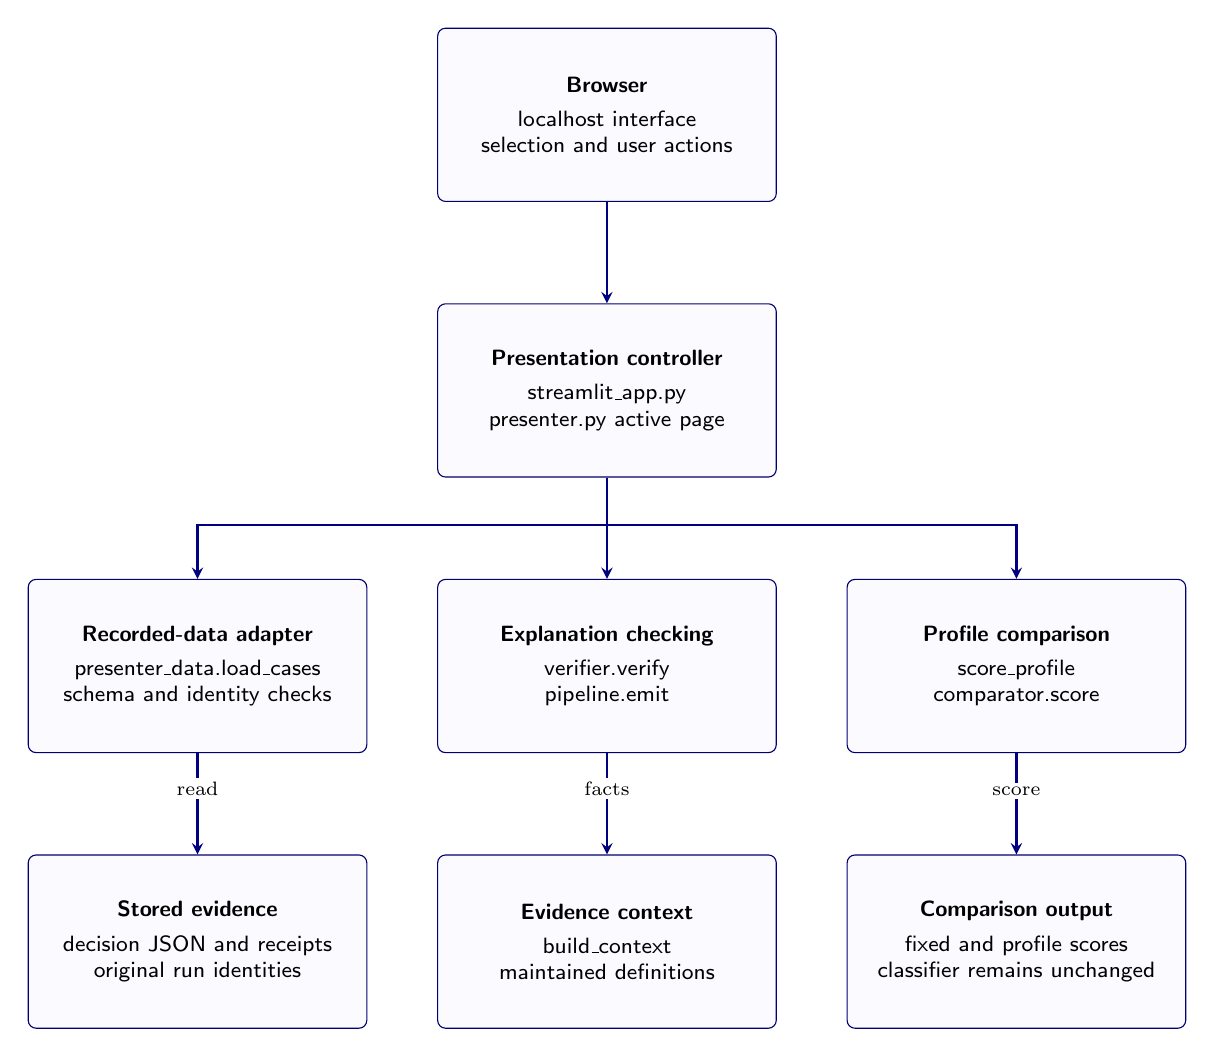
\begin{tikzpicture}[x=1mm,y=1mm,box/.style={draw=blue!45!black,fill=blue!2,rounded corners=1mm,align=center,text width=39mm,minimum height=22mm,inner sep=2mm,font=\sffamily\footnotesize},link/.style={->,>=stealth,draw=blue!50!black,thick}]
\node[box] (browser) at (75,140) {\textbf{Browser}\\[1mm]localhost interface\\selection and user actions};
\node[box] (presenter) at (75,105) {\textbf{Presentation controller}\\[1mm]streamlit\_app.py\\presenter.py active page};
\node[box] (loader) at (23,70) {\textbf{Recorded-data adapter}\\[1mm]presenter\_data.load\_cases\\schema and identity checks};
\node[box] (checking) at (75,70) {\textbf{Explanation checking}\\[1mm]verifier.verify\\pipeline.emit};
\node[box] (risk) at (127,70) {\textbf{Profile comparison}\\[1mm]score\_profile\\comparator.score};
\node[box] (artifacts) at (23,35) {\textbf{Stored evidence}\\[1mm]decision JSON and receipts\\original run identities};
\node[box] (context) at (75,35) {\textbf{Evidence context}\\[1mm]build\_context\\maintained definitions};
\node[box] (result) at (127,35) {\textbf{Comparison output}\\[1mm]fixed and profile scores\\classifier remains unchanged};
\draw[link] (browser.south) -- ++(0,-6) -| (presenter.north);
\draw[link] (presenter.south) -- ++(0,-6) -| (loader.north);
\draw[link] (presenter.south) -- ++(0,-6) -| (checking.north);
\draw[link] (presenter.south) -- ++(0,-6) -| (risk.north);
\draw[link] (loader.south) -- ++(0,-6) -| (artifacts.north) node[pos=.5,above,fill=white,inner sep=.5mm,font=\scriptsize]{read};
\draw[link] (checking.south) -- ++(0,-6) -| (context.north) node[pos=.5,above,fill=white,inner sep=.5mm,font=\scriptsize]{facts};
\draw[link] (risk.south) -- ++(0,-6) -| (result.north) node[pos=.5,above,fill=white,inner sep=.5mm,font=\scriptsize]{score};
\end{tikzpicture}
\caption{Implemented components and their interfaces.}\label{fig:components}\end{figure}
\begin{figure}[htbp]\centering\resizebox{\linewidth}{!}{\begin{tikzpicture}[x=1mm,y=1mm,b/.style={draw,text width=135mm,minimum height=23mm,align=center,font=\sffamily\footnotesize},>=Stealth]
\node[b] (ui) at (75,119){\textbf{Presentation}\\Overview / Decision / Evidence / Risk / Explanation / Studies};
\node[b] (app) at (75,81){\textbf{Application}\\Case loading, current-state ownership, confidence policy and emission};
\node[b] (domain) at (75,43){\textbf{Domain}\\Validated records, feature meanings, tolerance/capacity and claim checks};
\node[b] (files) at (75,5){\textbf{Artifacts / runtime}\\Versioned JSON traces, original models, study receipts and local session memory};
\draw[->](ui)--node[right,font=\scriptsize]{user action}(app);\draw[->](app)--node[right,font=\scriptsize]{validated contract}(domain);\draw[->](domain)--node[right,font=\scriptsize]{read / retain identity}(files);
\end{tikzpicture}}
\caption{Presentation, application, domain and artifact layers.}\label{fig:layers}\end{figure}
\section{Domain and Class Model}
The class model includes attributes and operations used by the code. Multiplicities distinguish a collection of records, a record's contributions and candidate/verification relationships. Profile evaluation is a dependency on a record, not a mutation of classifier probabilities.
\begin{figure}[p]\centering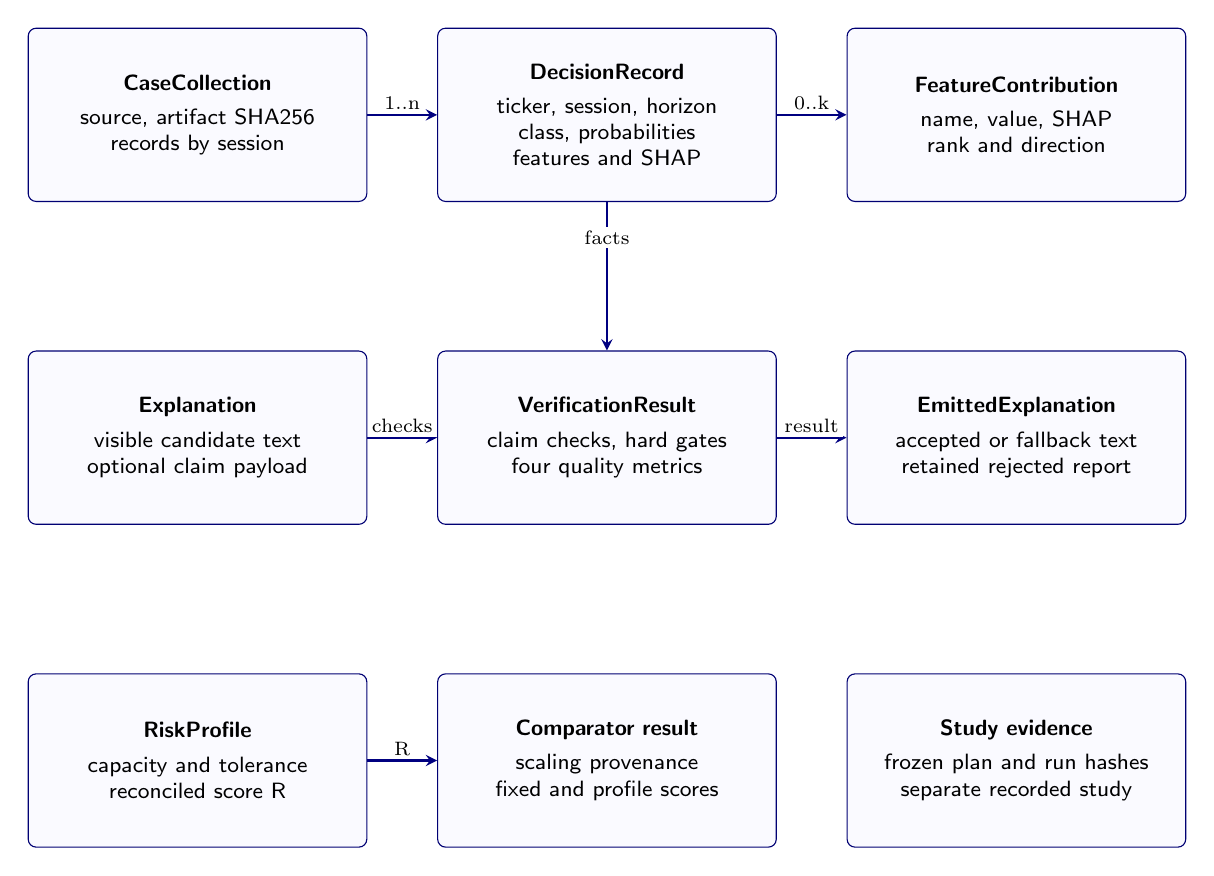
\begin{tikzpicture}[x=1mm,y=1mm,box/.style={draw=blue!45!black,fill=blue!2,rounded corners=1mm,align=center,text width=39mm,minimum height=22mm,inner sep=2mm,font=\sffamily\footnotesize},link/.style={->,>=stealth,draw=blue!50!black,thick}]
\node[box] (collection) at (23,100) {\textbf{CaseCollection}\\[1mm]source, artifact SHA256\\records by session};
\node[box] (record) at (75,100) {\textbf{DecisionRecord}\\[1mm]ticker, session, horizon\\class, probabilities\\features and SHAP};
\node[box] (contrib) at (127,100) {\textbf{FeatureContribution}\\[1mm]name, value, SHAP\\rank and direction};
\node[box] (explanation) at (23,59) {\textbf{Explanation}\\[1mm]visible candidate text\\optional claim payload};
\node[box] (verification) at (75,59) {\textbf{VerificationResult}\\[1mm]claim checks, hard gates\\four quality metrics};
\node[box] (emission) at (127,59) {\textbf{EmittedExplanation}\\[1mm]accepted or fallback text\\retained rejected report};
\node[box] (profile) at (23,18) {\textbf{RiskProfile}\\[1mm]capacity and tolerance\\reconciled score R};
\node[box] (comparison) at (75,18) {\textbf{Comparator result}\\[1mm]scaling provenance\\fixed and profile scores};
\node[box] (study) at (127,18) {\textbf{Study evidence}\\[1mm]frozen plan and run hashes\\separate recorded study};
\draw[link] (collection.east) -- (record.west) node[pos=.5,above,fill=white,inner sep=.5mm,font=\scriptsize]{1..n};
\draw[link] (record.east) -- (contrib.west) node[pos=.5,above,fill=white,inner sep=.5mm,font=\scriptsize]{0..k};
\draw[link] (record.south) -- ++(0,-6) -| (verification.north) node[pos=.5,above,fill=white,inner sep=.5mm,font=\scriptsize]{facts};
\draw[link] (explanation.east) -- (verification.west) node[pos=.5,above,fill=white,inner sep=.5mm,font=\scriptsize]{checks};
\draw[link] (verification.east) -- (emission.west) node[pos=.5,above,fill=white,inner sep=.5mm,font=\scriptsize]{result};
\draw[link] (profile.east) -- (comparison.west) node[pos=.5,above,fill=white,inner sep=.5mm,font=\scriptsize]{R};
\end{tikzpicture}
\caption{Implementation class model with attributes, operations and multiplicities.}\label{fig:classes}\end{figure}
\section{Data Flow and File Schema}
The schema identifies experiment and composite case identities, keyed feature maps, candidate digests and result ownership. These are JSON/file/session contracts, not a claimed SQL database. Relationship labels and cardinalities express how the actual loader and checker bind their data.
\begin{figure}[htbp]\centering\resizebox{\linewidth}{!}{\begin{tikzpicture}[x=1mm,y=1mm,b/.style={draw,rounded corners,text width=49mm,minimum height=24mm,align=center,font=\sffamily\footnotesize},store/.style={draw,double,text width=49mm,minimum height=19mm,align=center,font=\sffamily\footnotesize},>=Stealth]
\node[b] (user) at (75,146){User: selection, answers and candidate};\node[b] (loader) at (32,106){P1: load/validate\\Case + source identity};\node[b] (profile) at (118,106){P2: score profile/policy\\Capacity, tolerance, allowance};
\node[b] (check) at (32,61){P3: verify claims\\Candidate and source independently};\node[b] (emit) at (118,61){P4: emit current result\\Accepted, fallback or error};
\node[store] (files) at (32,13){D1: recorded artifacts / receipts};\node[store] (state) at (118,13){D2: session profile / result identity};
\draw[->](user.south)-|node[pos=.35,above,font=\scriptsize]{case/text}(loader.north);\draw[->](user.south)-|node[pos=.35,above,font=\scriptsize]{18 answers}(profile.north);
\draw[->](files.west)--(-5,13)--node[left,font=\scriptsize]{record}(-5,106)--(loader.west);\draw[->](loader)--(check);\draw[->](check)--node[above,font=\scriptsize]{verdict}(emit);\draw[->](profile)--node[right,font=\scriptsize]{policy result}(emit);\draw[->](emit)--(state);
\draw[->](emit.east)--(153,61)--(153,146)--node[above,font=\scriptsize]{current display}(user.east);
\end{tikzpicture}}
\caption{Data flow through the current checking and policy path.}\label{fig:dataflow}\end{figure}
\begin{figure}[p]\centering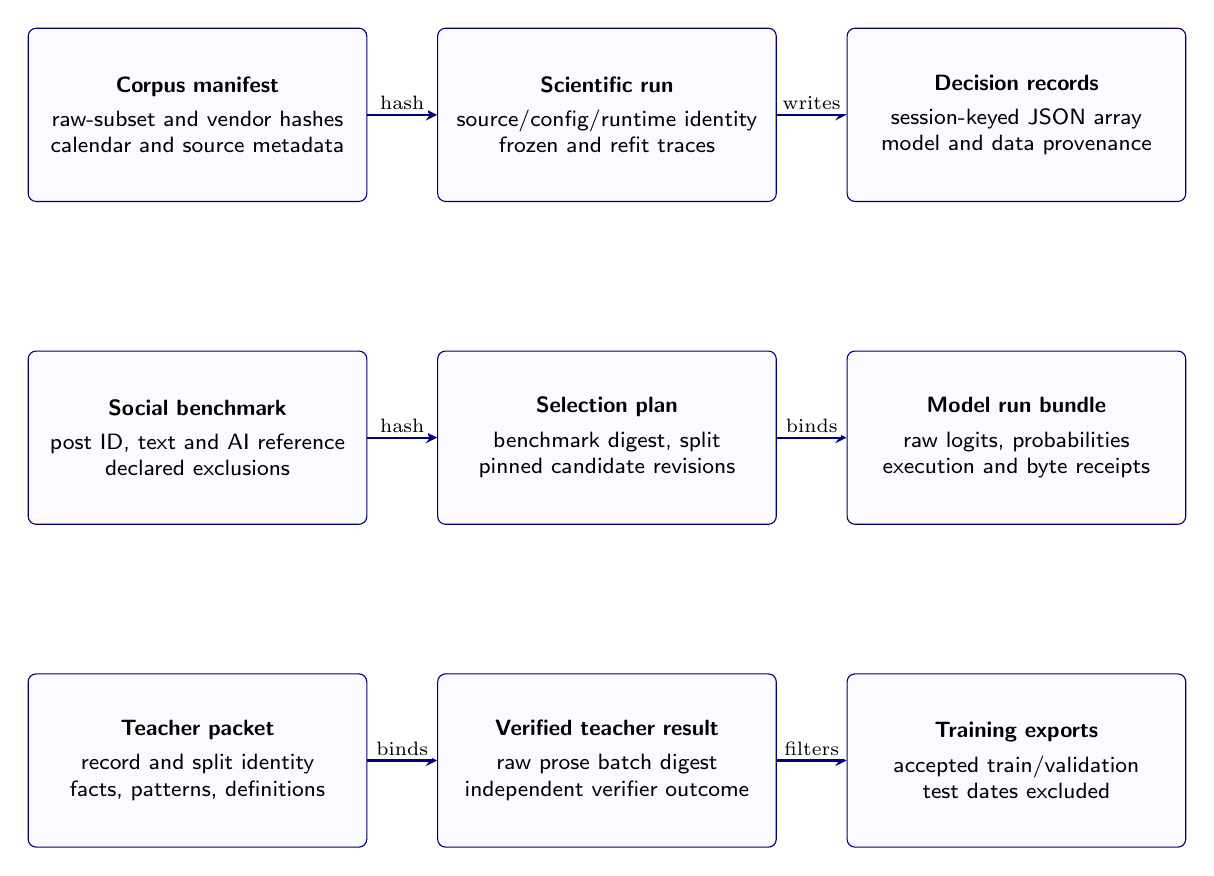
\begin{tikzpicture}[x=1mm,y=1mm,box/.style={draw=blue!45!black,fill=blue!2,rounded corners=1mm,align=center,text width=39mm,minimum height=22mm,inner sep=2mm,font=\sffamily\footnotesize},link/.style={->,>=stealth,draw=blue!50!black,thick}]
\node[box] (manifest) at (23,105) {\textbf{Corpus manifest}\\[1mm]raw-subset and vendor hashes\\calendar and source metadata};
\node[box] (run) at (75,105) {\textbf{Scientific run}\\[1mm]source/config/runtime identity\\frozen and refit traces};
\node[box] (records) at (127,105) {\textbf{Decision records}\\[1mm]session-keyed JSON array\\model and data provenance};
\node[box] (benchmark) at (23,64) {\textbf{Social benchmark}\\[1mm]post ID, text and AI reference\\declared exclusions};
\node[box] (plan) at (75,64) {\textbf{Selection plan}\\[1mm]benchmark digest, split\\pinned candidate revisions};
\node[box] (bundle) at (127,64) {\textbf{Model run bundle}\\[1mm]raw logits, probabilities\\execution and byte receipts};
\node[box] (packet) at (23,23) {\textbf{Teacher packet}\\[1mm]record and split identity\\facts, patterns, definitions};
\node[box] (teacher) at (75,23) {\textbf{Verified teacher result}\\[1mm]raw prose batch digest\\independent verifier outcome};
\node[box] (exports) at (127,23) {\textbf{Training exports}\\[1mm]accepted train/validation\\test dates excluded};
\draw[link] (manifest.east) -- (run.west) node[pos=.5,above,fill=white,inner sep=.5mm,font=\scriptsize]{hash};
\draw[link] (run.east) -- (records.west) node[pos=.5,above,fill=white,inner sep=.5mm,font=\scriptsize]{writes};
\draw[link] (benchmark.east) -- (plan.west) node[pos=.5,above,fill=white,inner sep=.5mm,font=\scriptsize]{hash};
\draw[link] (plan.east) -- (bundle.west) node[pos=.5,above,fill=white,inner sep=.5mm,font=\scriptsize]{binds};
\draw[link] (packet.east) -- (teacher.west) node[pos=.5,above,fill=white,inner sep=.5mm,font=\scriptsize]{binds};
\draw[link] (teacher.east) -- (exports.west) node[pos=.5,above,fill=white,inner sep=.5mm,font=\scriptsize]{filters};
\end{tikzpicture}
\caption{Artifact/session schema with keys and relationship cardinalities.}\label{fig:schema}\end{figure}
\section{Behavioral Design}
The sequence starts with the actual Check explanation click and uses alternative fragments for acceptance and recovery. The activity includes invalid input and fallback-verification failure. The state model includes initialization, stale results, errors and session termination.
\begin{figure}[p]\centering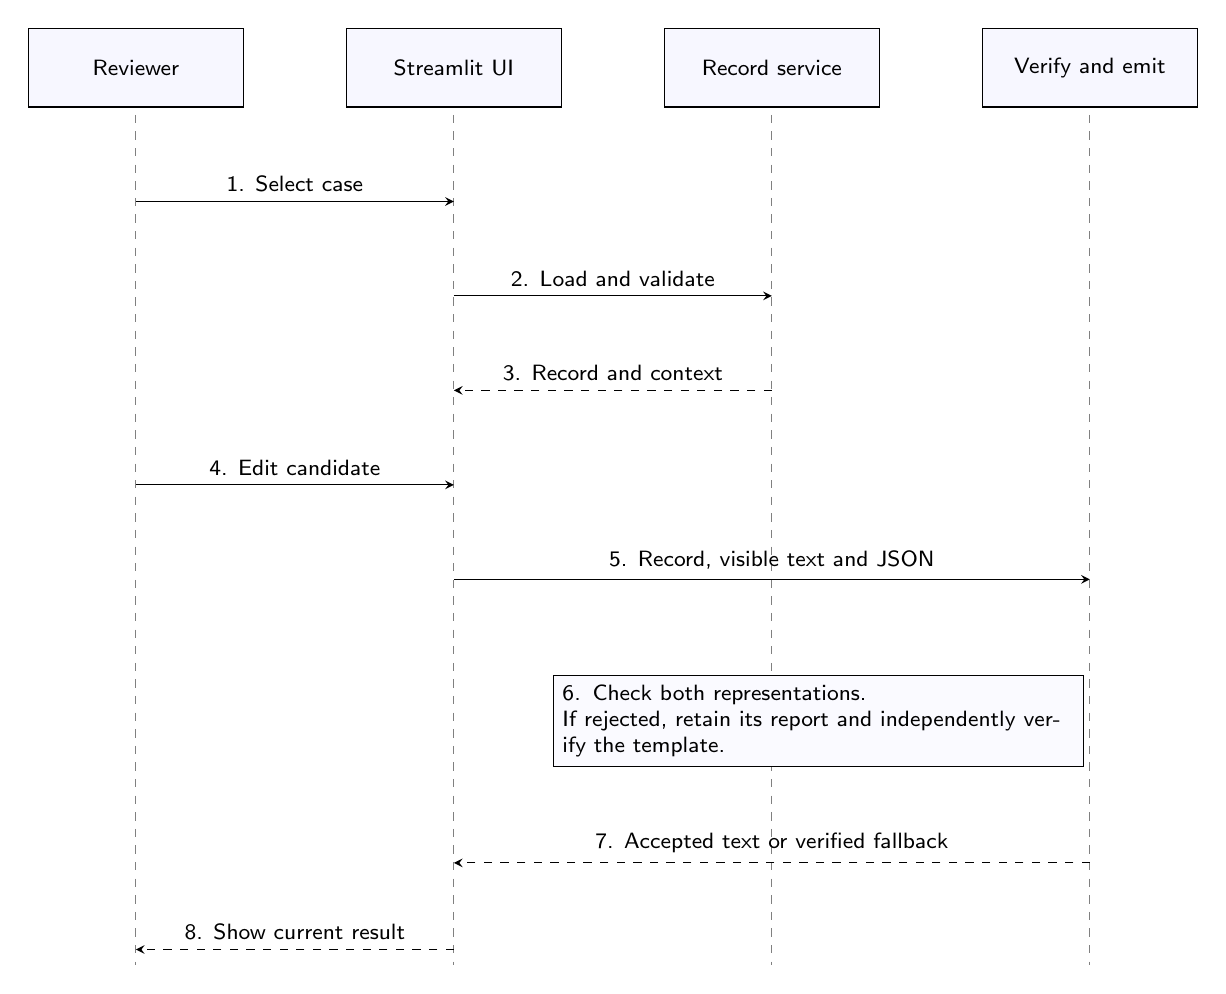
\begin{tikzpicture}[x=.985mm,y=1mm,font=\sffamily\footnotesize,>=stealth]
\foreach \x/\n in {12/Reviewer,53/Streamlit UI,94/Record service,135/Verify and emit}{
\node[draw,fill=blue!3,text width=25mm,align=center,minimum height=10mm] at (\x,122){\n};
\draw[dashed,gray] (\x,116)--(\x,8);}
\draw[->] (12,105)--node[above]{1. Select case}(53,105);
\draw[->] (53,93)--node[above]{2. Load and validate}(94,93);
\draw[->,dashed] (94,81)--node[above]{3. Record and context}(53,81);
\draw[->] (12,69)--node[above]{4. Edit candidate}(53,69);
\draw[->] (53,57)--node[above]{5. Record, visible text and JSON}(135,57);
\node[align=left,text width=65mm,fill=blue!2,draw] at (100,39){6. Check both representations.\\If rejected, retain its report and independently verify the template.};
\draw[->,dashed] (135,21)--node[above]{7. Accepted text or verified fallback}(53,21);
\draw[->,dashed] (53,10)--node[above]{8. Show current result}(12,10);
\end{tikzpicture}
\caption{Explanation-check sequence with explicit user trigger and alternative outcomes.}\label{fig:sequence}\end{figure}
\begin{figure}[p]\centering\resizebox{\linewidth}{!}{\begin{tikzpicture}[x=1mm,y=1mm,b/.style={draw,rounded corners,text width=48mm,minimum height=15mm,align=center,font=\sffamily\footnotesize},d/.style={draw,diamond,aspect=2.5,align=center,font=\sffamily\scriptsize,inner sep=1mm},>=Stealth]
\node[circle,fill,minimum size=3mm,inner sep=0] (start) at (75,192){};
\node[b] (load) at (75,175){Load and validate selected record};\node[d] (valid) at (75,151){Valid?};
\node[b] (candidate) at (75,126){Read current text/payload; verify independently};\node[d] (pass) at (75,101){Candidate passes?};
\node[b] (accept) at (28,76){Emit candidate and accepted report};\node[b] (fallback) at (122,76){Retain rejection; render fallback};
\node[d] (fallbackpass) at (122,46){Fallback passes?};\node[b] (emit) at (76,18){Emit checked replacement};\node[b] (error) at (20,18){Show error; no verified output};
\node[circle,draw,double,fill=black,minimum size=4mm,inner sep=0] (end) at (75,-11){};
\draw[->](start)--(load);\draw[->](load)--(valid);\draw[->](valid)--node[right]{yes}(candidate);\draw[->](candidate)--(pass);
\draw[->](valid.west)--node[above]{no}(-15,151)--(-15,18)--(error.west);
\draw[->](pass.west)-|node[pos=.25,above]{yes}(accept.north);\draw[->](pass.east)-|node[pos=.25,above]{no}(fallback.north);
\draw[->](fallback)--(fallbackpass);\draw[->](fallbackpass.south)|-node[pos=.25,above]{yes}(emit.east);
\draw[->](fallbackpass.east)--node[above]{no}(154,46)--(154,0)--(20,0)--(error.south);
\draw[->](accept.south)--(28,55)--(-30,55)--(-30,-11)--(end.west);
\draw[->](emit.south)--(end.north);\draw[->](error.south)|-(end.west);
\end{tikzpicture}}
\caption{Checking activity, including verified fallback and error termination.}\label{fig:activity}\end{figure}
\begin{figure}[p]\centering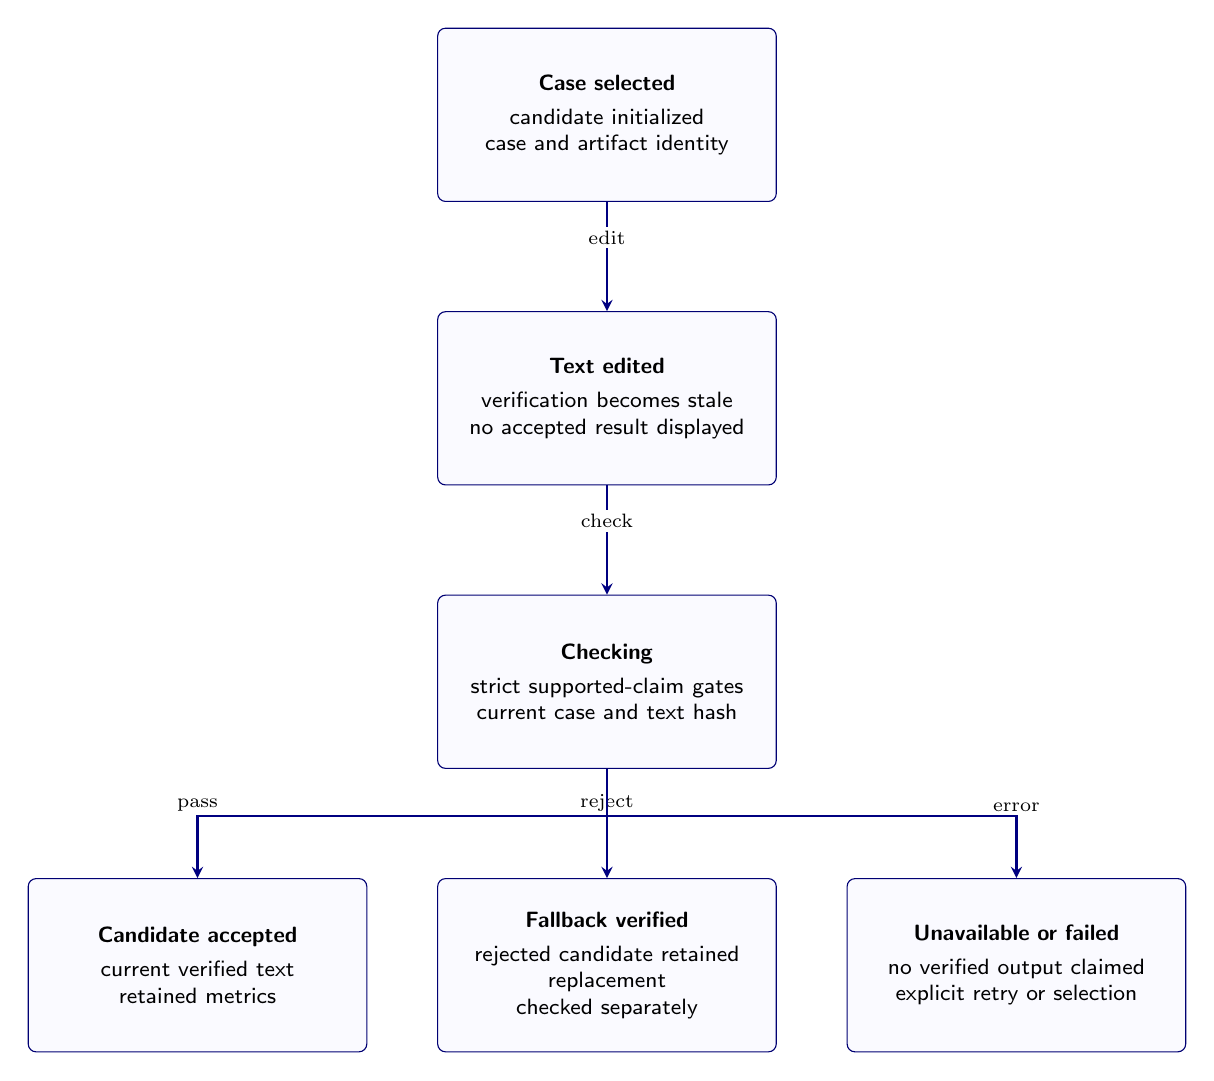
\begin{tikzpicture}[x=1mm,y=1mm,box/.style={draw=blue!45!black,fill=blue!2,rounded corners=1mm,align=center,text width=39mm,minimum height=22mm,inner sep=2mm,font=\sffamily\footnotesize},link/.style={->,>=stealth,draw=blue!50!black,thick}]
\node[box] (selected) at (75,135) {\textbf{Case selected}\\[1mm]candidate initialized\\case and artifact identity};
\node[box] (edited) at (75,99) {\textbf{Text edited}\\[1mm]verification becomes stale\\no accepted result displayed};
\node[box] (checking) at (75,63) {\textbf{Checking}\\[1mm]strict supported-claim gates\\current case and text hash};
\node[box] (accepted) at (23,27) {\textbf{Candidate accepted}\\[1mm]current verified text\\retained metrics};
\node[box] (fallback) at (75,27) {\textbf{Fallback verified}\\[1mm]rejected candidate retained\\replacement checked separately};
\node[box] (error) at (127,27) {\textbf{Unavailable or failed}\\[1mm]no verified output claimed\\explicit retry or selection};
\draw[link] (selected.south) -- ++(0,-6) -| (edited.north) node[pos=.5,above,fill=white,inner sep=.5mm,font=\scriptsize]{edit};
\draw[link] (edited.south) -- ++(0,-6) -| (checking.north) node[pos=.5,above,fill=white,inner sep=.5mm,font=\scriptsize]{check};
\draw[link] (checking.south) -- ++(0,-6) -| (accepted.north) node[pos=.5,above,fill=white,inner sep=.5mm,font=\scriptsize]{pass};
\draw[link] (checking.south) -- ++(0,-6) -| (fallback.north) node[pos=.5,above,fill=white,inner sep=.5mm,font=\scriptsize]{reject};
\draw[link] (checking.south) -- ++(0,-6) -| (error.north) node[pos=.5,above,fill=white,inner sep=.5mm,font=\scriptsize]{error};
\end{tikzpicture}
\caption{Case/candidate verification state transitions.}\label{fig:state}\end{figure}
\section{Deployment and Design Evolution}
The localhost browser communicates with Streamlit. Core modules read registered artifacts and retain profile/candidate state in memory. CI produces downloadable review artifacts; it does not host the application. The revised deployment model includes the core-to-artifact link.
\begin{figure}[htbp]\centering\resizebox{\linewidth}{!}{\begin{tikzpicture}[x=1mm,y=1mm,b/.style={draw,rounded corners,text width=62mm,minimum height=27mm,align=center,font=\sffamily\footnotesize},>=Stealth]
\node[b] (browser) at (75,146){\textless\textless device\textgreater\textgreater\\Browser on project/groupmate laptop};
\node[b] (server) at (75,96){\textless\textless execution environment\textgreater\textgreater\\Python 3.11 / Streamlit, loopback 8507\\Presenter + core context/profile/verifier};
\node[b] (files) at (33,40){\textless\textless artifact\textgreater\textgreater\\Recorded cases, traces and study receipts};\node[b] (memory) at (117,40){\textless\textless session state\textgreater\textgreater\\Profile, candidate and current result};
\draw[->](browser)--node[right,font=\scriptsize]{HTTP / WebSocket}(server);
\draw[->](server.south)-|node[pos=.25,above,font=\scriptsize]{core reads}(files.north);\draw[->](server.south)-|node[pos=.25,above,font=\scriptsize]{local state}(memory.north);
\node[draw,dashed,text width=137mm,align=center,font=\sffamily\footnotesize,inner sep=3mm] (ci) at (75,-5){GitHub Actions: Windows/Ubuntu checks $\rightarrow$ verified downloadable source/PDF artifact. Production hosting and trained-student serving are later deployment targets.};
\draw[->,dashed](ci.north west)--node[left,font=\scriptsize]{clone / extract}(files.south west);
\end{tikzpicture}}
\caption{Current localhost deployment and artifact-delivery boundary.}\label{fig:deployment}\end{figure}
The proposal's broad product design is retained, while the implemented slice now has complete evidence, independent prose/JSON checks, a full scored profile and uncertainty gating. The prior risk-dependent sentiment blend and isotonic outputs remain historical comparisons. Broader conversation, social divergence and production service work are explicitly scheduled.
\section{Algorithms and Contracts}
Record validation precedes display. Checking retains candidate errors, constructs fallback and verifies it independently. Temperature fitting admits only earlier-matured calibration labels. Profile scoring validates every answer, calculates weighted capacity/caps and published item totals, reconciles restrictive limits and evaluates confidence without changing direction. Each boundary carries identity and failure conditions used by its tests.

\chapter{Iteration 1: Design and Implementation}
\section{Iteration Objectives}
Preserve the existing project, validate the cached decision/explanation path, and make technical/news evidence inspectable. Establish the LLM input boundary and replay six recorded assistant-teacher examples; a live generator and measured user-comprehension benefit remain pending.

\section{Selected Use Cases / Features}
Select a historical corpus/session, inspect the decision/probabilities, read every feature's meaning and attribution, and inspect coverage/limitations. Fault checks reject corrupted confidence and show verified fallback.

\section{Design}
The frozen decision record remains the prediction source. A new builder combines its facts with reviewed definitions and implementation limitations. Streamlit and the standalone explorer reuse that context. Existing template verification remains the baseline.

\section{Implementation}
The independent code copy is on branch \texttt{gpt/mid-eval}. New code in \texttt{src/investify/explain/context.py} covers every feature, handles missing values, rejects non-finite attributions/probabilities, and identifies unreviewed definitions. The Decision tab renders the context; the exporter uses the same records.

\section{Completed Features / Module}
The context, artifact tools, complete-guided verifier, report-retaining fallback, both live interfaces, prototype profile and separate retrospective risk comparator are implemented. Actual Streamlit widget tests pass. Six actual teacher explanations are saved and replayed in Teacher Study. Live model inference, candidate social-model comparison, social features, personalized classifier predictions and remote GitHub execution remain pending.

\section{Technical Implementation Details}
Feature values and predicted-class SHAP contributions are separate. Family totals retain raw-score units. The verifier checks prose and JSON independently, including feature values and attribution targets. Displayed-text coverage, essential disclosures and hard contradiction gates prevent a correct payload from hiding an incorrect display. Strict mode rejects unsupported sentences. Evidence tools check schemas/context/templates/distributions/additivity and record artifact/runtime/source hashes.

\section{Algorithms and Technical Decisions}
Definitions follow actual features: dispersion is trailing variation of session-average polarity, and news attention is a headline-count z-score. Missing data stays missing. Indicator meaning and its use by this model are distinct \cite{fidelity_rsi,fidelity_macd,fidelity_obv}.

\section{Tools, Frameworks and Technologies}
The portable path uses standard Python. The restored isolated viewer/test environment yields 212 selected passes and no skips; it is not the locked scientific environment. CI targets Python 3.11 on Windows/Linux with portable checks, frozen plans, comparator audits and a separate Streamlit AppTest job. Remote jobs have not run.

\section{Demonstration Evidence}
The continuation adds an explicitly labelled feature-level causality button: nine checks on synthetic fixtures detect four centred-window mutations, with no classifier fit. Scientific input/runtime absence disables the real re-run, and a later import/data failure is reported without a fabricated experiment result. Portable reports are invalidated after candidate/settings edits; record-loading errors retain selection/retry controls. These checks are distinct from browser visual QA.
Artifact checks cover 186 records per corpus. The live HTTP exercise passes 62 explanation/risk cases. The separate comparator audit passes 228 arithmetic checks on actual held-out rows with labelled parameter scenarios. Browser visual QA remains pending. Both saved classifiers predict Buy throughout; no predictor-performance improvement is claimed.

\section{Iteration Outcome}
\subsection{Versioned Scientific Corrections}
The historical purger used calendar-day subtraction for observed-row labels. On the same labelled business-day fixture/test blocks it retains 18 training-label endpoints reaching the evaluation blocks; the corrected \texttt{observed-label-end-purge-v2} retains zero. Actual endpoints are calculated before feature filtering and carried to folds. Calibration candidates ending on/after first evaluation are excluded; a future-price shock leaves retained fixture inputs unchanged. Explicit frozen-classifier and refit-transfer modes now support a fair source-level comparison, but actual model fitting/results require restored inputs/runtime.

Original scientific source/results are preserved. Cache joins refuse duplicate document keys or inconsistent probabilities, RSI edge windows have explicit behaviour, datetime units are normalized for the as-of join, and input ranges/ticker/revision/calendar contracts fail visibly. New outputs/cache directories are isolated. Full score/margin/truth arrays, calibration knots, scaler/model bytes and source/input identity are retained by the new trace mechanism. None of these source/fixture repairs establishes changed historical performance or explains the all-Buy result. E\_SAMEBAR\_TEXT is a lag-rule ablation under the retained strict-prior join.
The increment improves evidence coverage and transparency over the top-k numeric template and supplies a tested LLM input contract. It does not yet establish LLM usefulness, predictive skill, complete mid readiness, or deployment.

\section{Recorded Assistant Teacher Construction Pilot}
Under the user's latest direction, the current assistant supplies teacher examples before an alternative API is considered. The planned student remains Phi-3-mini; no additional Qwen teacher download is required. Six actual explanations were written from frozen historical NVDA records, and all six pass the current strict verifier. Input packets contain facts, reviewed definitions and controlled sentence patterns without a completed reference answer.

The supervision is hybrid: prose is actually assistant-generated, while the factual JSON payload is assembled deterministically from the original record. Both are checked, but the payload is not claimed as a teacher completion. Exact serving model ID/revision, decoding, token usage and per-example inference latency are unavailable and recorded as null.

Both corpora share date groups: 118 training dates, 30 validation dates and 38 preserved held-out test dates. The actual pilot has four training and two validation examples; test records are excluded. All saved source decisions are Buy, so neither class generalization nor adequate QLoRA data is established. Some held-out examples were previously explored; no first-ever untouched-test claim is made. Copied evidence replays original hash-bound raw persistence times and exact exports.

Original-student inference, QLoRA training, student quality and user understanding remain unmeasured. The inspected GPU has 10,240 MiB; the proposal's 16 GB envelope does not establish current-machine feasibility. Required training libraries, exact student checkpoint/tokenizer and measured token/VRAM budgets remain pending. Earlier Qwen-specific local pilot choices are inactive for the selected teacher/student workflow.

\chapter{Testing and Early Validation}
\label{chap:testing}
\section{Strategy and Test Levels}
Unit tests exercise validation, formulas and hard rejection gates. Module tests combine records, evidence, profiles and emitted explanations. Streamlit AppTest exercises actual widgets; a localhost HTTP exercise validates the portable pipeline. Source/receipt guards and clean extraction verify artifact reproducibility. Scientific execution and classifier sanity probes are separate from software fixtures.
\section{Evaluation Metrics Matrix}
\begin{longtable}{p{0.18\textwidth}p{0.27\textwidth}p{0.26\textwidth}p{0.18\textwidth}}
\caption{Metrics, evaluation population and measured/planned status.}\label{tab:metrics-matrix}\\\toprule Area & Measures & Evaluation population/protocol & Status\\\midrule
Prediction & Macro-F1, per-class precision/recall, baseline lift & NVDA chronological folds; random and linear comparators & Measured; weak signal\\
Calibration & Brier, class distribution, negative log likelihood & Earlier calibration labels; same 186 evaluation cases & Measured; abstention required\\
Leakage & Control lift/intervals, boundary/fault detection & Six arms, two horizons, fixed folds/settings & Measured; labelled canary fires\\
Explanation & Numeric/directional fidelity, recall, unverifiable rate; rejection/fallback & Saved cases, deliberate corruptions and construction pilot & Bounded behavior measured; larger generation study later\\
Social sentiment & Macro-F1 agreement, per-class recall, coverage & Same 24 held-out target-equity references & Exploratory comparison measured\\
User understanding & Task completion/time, interpretation errors, top-driver identification & Planned participant tasks and expert review & Later evaluation\\
System & Latency, memory, throughput, parity and setup & Specified target environment and clean-host paths & Setup/path checks measured; target NFRs later\\
\bottomrule\end{longtable}
\section{Current Software Checks}
The current revision adds calibration-availability/rank tests and full-profile scoring/policy tests. Existing corruption, record, transport and interface regressions remain. Named input/expected/actual cases are listed in Appendix~\ref{app:tests}; final scoped receipts record the exact executed counts. Historical counts are not repeated as if they were one current suite. The hosted matrix proves its committed snapshot; new local changes require their own checks before publication.
\section{Social Study and Diagnostic Probes}
\begin{longtable}{p{0.32\textwidth}p{0.28\textwidth}p{0.29\textwidth}}
\caption{Social study population, split and original-classifier outcomes.}\label{tab:social-study}\\\toprule Item & Value & Interpretation\\\midrule
Acquired / usable / excluded & 200 / 117 / 83 & Exclusions are retained with reasons\\
Usable reference classes & 31 positive / 67 neutral / 19 negative & Imbalanced target-equity references\\
Development / held out & 93 / 24 & Frozen chronological selection\\
Held-out classes & 7 positive / 15 neutral / 2 negative & Negative recall moves in 50-point steps\\
CryptoBERT & Macro-F1 0.2564; exact 15/24 & All held-out predictions neutral\\
Cardiff & Macro-F1 0.6016; exact 16/24 & Exploratory leader, not final deployment selection\\
\bottomrule\end{longtable}
The reference-construction method is disclosed in Appendix~\ref{app:handbook}. Scores measure agreement with that reference, not independent human-validated accuracy or NVDA return prediction.

A new offline sanity check uses five authored crypto-text probes, kept separate from the frozen equity benchmark. The original CryptoBERT checkpoint returns both positive and negative classes: the two intended-positive and two intended-negative probes match their diagnostic direction. The nominal neutral probe returns negative. This rules out an invariant neutral output on every input, while showing the probes are not a validated accuracy set. We retain the original 24-post result and do not relabel the benchmark to improve it.
\section{Failure and Recovery Evidence}
The demonstration pairs correct factual text with a deliberately incorrect visible probability beside correct JSON. The candidate fails and the checked fallback retains the authoritative probability. Edits/case changes remove stale verification. Missing records, partial model outputs and invalid profiles withhold replacements. Temperature calibration preserves raw class order; actual near-uniform confidence abstains under both profile extremes. Controlled 0.70-confidence Buy/Sell cases demonstrate that allowance changes abstention without reversing direction or mutating probabilities.
\section{Defects Corrected}
Corrections address payload-over-prose acceptance, missing/non-top-k evidence checks, retained rejection reporting, stale state, label-endpoint purging, calibration-outcome availability, and platform-specific provenance-path handling. The present revision adds multiclass diagnosis/abstention and replaces risk-dependent sentiment weighting in the primary interface. Old model/data/label artifacts remain separately identified.
\section{Validation Boundary}
The live module and engineered failures are observable and tested. Predictor usefulness, unrestricted generated-text quality, population-specific suitability and participant comprehension are separate evaluation goals. Physical rehearsal/projector checks and formal meeting/signature records remain team activities.

\chapter{Project Management and Development Evidence}
\section{Work Completed}
The isolated copy preserves original history/documents. Completed work includes complete feature/family evidence, independent prose/JSON checks, strict mode, rejection/fallback reporting, local LLM transport/evaluation plumbing, both live interfaces, restored viewer runtime, authoritative-record validation, an explicit prototype profile and a separate retrospective risk comparator. The selected suite has 212 passes and no skips; local evidence covers 372 records, 62 live HTTP cases and 228 comparator arithmetic probes. CI jobs are prepared.
\section{Work Remaining}
The real fresh Alpaca scientific run and original-publisher paired social comparison now complete, with retained raw execution, source/input identity and replay evidence. Cardiff leads the small AI-reference benchmark; final adequacy criteria, independent validation and deployment selection remain open. Source/raw labels, exclusions and the original V3 chronology are preserved.

Current gaps are institutional report/deck inspection and completion, genuine member contributions and review/rehearsal, current repository/remote CI evidence, live LLM usefulness and agreed risk semantics. The original September bytes and exact scientific lock are not reproduced. Student inference/training and broader acceptance work remain later milestones.

\section{Contribution of Each Team Member}
Section~\ref{sec:planned-work-division} contains the proposal's planned member assignments. Ahmed covers the point-in-time harness, leakage/timestamp/parity work and deployment; Rafay covers risk profiling, sentiment, degraded operation, acceptance and frontend; Soban covers the decision engine, calibration, SHAP, verifier and later QLoRA. Each member must record actual implementation, review, testing and defence preparation. The planned table does not establish completion or authorship of assistant-supported work.
\section{Repository and Version Control Evidence}
The consolidated repository is on \texttt{main}. Original baseline \texttt{1dc24e0} and its isolated branch are preserved in history; local commit \texttt{93d0d60} records the fresh scientific increment. Current verification evidence records source/data hashes. Upstream access remains unverified; local workflow configuration is not evidence of a successful remote CI run.
\section{Continuous Integration and Delivery Status}
The GitHub Actions configuration runs two Python 3.11 jobs on Windows and Ubuntu after a push, pull request or manual dispatch. Both call the same versioned \texttt{run\_mid1\_ci.py} entry point used for local replay. The portable job executes standard-library regressions, saved-record validation, preview generation, a plan-only explainer check, comparator arithmetic and a real localhost HTTP exercise. The UI job runs scoped source checks and the legacy, presenter and recorded-study selector suites. Each retains logs and a byte-bound source/artifact receipt; CI artifacts are configured for fourteen-day retention.

The Windows local replay passes both jobs: 165 portable tests and seven CI source-ownership/metadata guards, 62 live HTTP checks, 372 validated historical records and 228 comparator probes, plus 42 UI tests in separate overlapping scopes. Temporary component metadata is restored after each job. The replay uses the already prepared local runtime; it does not establish a fresh dependency installation or Ubuntu/GitHub execution. The consolidated repository still has no configured remote. Actual remote CI remains open, and no continuous deployment, hosting target, model training or paid inference is executed by this workflow.
\section{Milestones and Commit Evidence}
The checkpoint distinguishes the initial context increment from verifier/local-demo work. Historical experiments are preserved separately from current test/HTTP evidence. Reproduction instructions appear in the repository appendix.
\section{Tools and Tool-Assisted Development}
The coding assistant contributed code, regression tests, drafts and programmatic validation. Earlier handoffs declare GPT-6.1 Sol/Xhigh as selected session configuration; the exact serving revision is not provider-authenticated. Student review, source verification, institutional declarations and accurate tool disclosure remain necessary. Student authorship is not inferred from assistant work.
\section{External Components and Dependencies}
The baseline uses FinBERT, XGBoost, isotonic calibration, TreeSHAP and Streamlit. The portable demo uses standard Python HTTP/JSON facilities and existing record/verifier code. The retained social labels were generated by the assistant in one actual session pass and disclosed as AI references. Six recorded assistant-teacher explanation completions are retained separately. No API/local student inference or human annotation is claimed.
\section{Risks and Mitigation}
Both interfaces expose recorded evidence and failure cases. The restored scientific runtime executes a separate fresh snapshot; original-byte and exact-lock limitations remain disclosed. Unknown deadline/owners affect scheduling; unavailable model access prevents measuring LLM usefulness. Constant-Buy classifier output prevents a predictive-skill claim. Prototype profile-to-blend assumptions require review and do not establish suitability.
\section{Security and Privacy Considerations}
The local demo serves historical decisions on loopback and has no trading/account access. Profile persistence, production authentication and deployment security are beyond this increment.
\section{Current Limitations}
Physical projector review, remote GitHub CI, real LLM evaluation, personalised classifier modelling and deployment remain pending. The current browser journey and compiled report/deck layouts have separate review receipts. New science and the original social-classifier comparison are recorded separately. The risk comparator remains an unvalidated prototype. Institutional metadata, signatures, genuine team review and remaining research are incomplete.

\section{Teacher Pilot Evidence}
The six recorded examples, four-training/two-validation split, serving-identity limitations and untrained Phi-3-mini student are documented once in Section~\ref{sec:teacher-pilot}. No training efficacy or human-comprehension result is inferred.

\chapter{Remaining FYP Plan}
\section{Remaining Scope}
Complete the broader stock research workflow, evaluate its contributions and document its operational boundaries. Brokerage execution remains excluded.
\section{Remaining Modules and Features}
Add audited company coverage, paired news/social features and divergence, a service layer, prompted explanations with constrained claims and optional verified student adaptation. Review the profile wording and the actual-close timing policy.
\section{Remaining Iterations}
Iteration 2 completes engine/service and the preregistered divergence comparison. Iteration 3 (Mid-2) adds the prompted explainer, free-prose claim binding, NFR/parity/degraded-operation measurement and acceptance preparation. Iteration 4 compares original and QLoRA-adapted Phi-3-mini with the template and performs broader evaluation and handover.
\section{Implementation Plan}
First audit additional source coverage and available-label boundaries. Freeze the divergence protocol before evaluating variants. Load a verified original student checkpoint, score its raw prompted baseline, expand filtered examples and preserve the held-out set before adaptation. Integrate the tested service and interface incrementally.
\section{Testing and Validation Plan}
Repeat the timing/canary controls for each scientific identity. Compare macro-F1, baseline lift, Brier/reliability and class distributions under shared splits. Measure raw and gated explanation quality. Inject missing feeds/thin history and pin a historical clock for serving parity. The automated workflow is \textbf{2 jobs $\times$ 2 OS = 4 checks, then 1 gated delivery job}; local counts remain distinct from classifier or participant evidence.
\section{Deployment Plan}
Prepare a container and an explicit target VM, measure the required environments and deploy the research service. Test installation from the documented package on a separate machine. Current CI delivers downloadable source/PDF artifacts; it does not deploy a production service.
\section{Tentative Timeline}
Use the proposal's relative checkpoints in Table~\ref{tab:engineering-dates}. Formal assessment appointments have not been supplied. Engine/divergence/service work precedes the Mid-2 prompted explainer, and QLoRA follows a working prompted baseline.
\section{Expected Final Deliverables}
Deliver integrated source/service, source-bound experiments and ablations, timing/calibration and explanation evaluations, measured performance/degraded-operation evidence, external installation instructions, participant records where completed, and final report/presentation. Retain a defensible null-result report if the learned engine has no useful advantage.

\chapter{Conclusion}
Investify Mid-1 implements an inspectable historical research flow with timing controls, complete evidence, a scored profile, deterministic explanation checking and verified recovery. The retained experiments show weak prediction, an isotonic class collapse and temperature confidence near one-third. The interface therefore presents Observe rather than a directional recommendation.

The revision responds to PF-01--PF-09 through explicit contributions, a scheduled LLM design, model/metric tables, market background, transparency acceptance and a demonstrable core. The next work is integrated divergence, useful prediction/calibration evaluation, the Mid-2 prompted explainer and operational/user validation. QLoRA remains Iteration 4.


\appendix
\chapter{Proposal Action Register}
\label{app:actions}
The original supplied comments remain preserved in the source register. This table records the concrete response and the work that still requires evaluation.
\begingroup\small
\begin{longtable}{p{0.12\textwidth}p{0.29\textwidth}p{0.48\textwidth}}
\caption{Proposal actions and current implementation response.}\label{tab:panel-actions}\\\toprule ID & Requested change & Response / remaining evaluation\\\midrule
PF-01 & Clear contribution & Harness and verifier separated from imported components; closest-work review remains\\
PF-02 & LLM benefit & Rich evidence contract, teacher construction and planned comparison; participant benefit unmeasured\\
PF-03 & Technical/sentiment explanation & All feature evidence and checked claims; integrated social evidence remains later\\
PF-04 & Refined problem & Educational interpretation, temporal evaluation and factual consistency\\
PF-05 & Model clarity & FinBERT news, evaluated social alternatives, frontier teacher construction and planned student\\
PF-06 & Metrics & Explicit matrix in Table~\ref{tab:metrics-matrix}; measured/planned status distinguished\\
PF-07 & Improved PoC & Live corruption/recovery, full profile, uncertainty gate and revised interface/design\\
PF-08 & Transparency & Historical data, weak confidence, failed calibration, method/scope and fallback disclosed\\
PF-09 & Market understanding & Timing, split/vintage, indicator meanings and attribution limits connected to design\\
\bottomrule\end{longtable}
\endgroup

\chapter{Detailed Requirements}
\begin{longtable}{p{0.16\textwidth}p{0.34\textwidth}p{0.39\textwidth}}
\toprule Requirement & Component & Evidence\\\midrule
MID-FR-01 & Schema/catalogue/input handling & Actual-record and missing/invalid-input checks\\
MID-FR-02 & Context and both interfaces & All 372 records; complete coverage tests\\
MID-FR-03 & Verifier & Prose/payload contradiction regressions\\
MID-FR-04 & Verifier/emission & Hard gates, omissions, malformed claims, verified fallback\\
MID-FR-05 & Emission/reporting & Retained failed report and HTTP assertions\\
MID-FR-06 & Strict prose gate & Clean acceptance and unsupported-sentence rejection\\
MID-FR-07 & Structural readiness/UI control & Missing, empty, truncated, invalid-type and read-denied fixtures; module discovery and actual widget checks\\
MID-FR-08 & Local adapter and interfaces & Retry, unavailable-provider, malformed/truncated output, loopback transport and fallback tests\\
MID-FR-09 & Guided template and verifier & All 372 guided records; modified-definition and coverage checks\\
MID-FR-10 & Evaluation command & Disjoint chronological selection, plan-only and zero-completion tests\\
MID-FR-11 & Complete guided contract & Non-top-k, missing/zero, family, target, scope and two-source coverage tests\\
MID-FR-12 & Prototype profile/form & All 32,400 answer combinations; cap, incomplete-answer and actual widget tests\\
MID-FR-13 & Retrospective scaling & Both 148/38 splits, held-out perturbation and development/missing-input refusal\\
MID-FR-14 & Separate comparator & Actual HTTP/AppTest independence; 228 real-row/labelled-scenario arithmetic checks\\
MID-FR-15 & Social-study provenance/plan & Fixture provenance checks plus the actual frozen 200-post/117-reference AI study\\
MID-FR-16 & Sentiment comparison tool & Matched-plan, per-model coverage/refusal, null partial metrics and explicit ties/raw-output tests; actual paired 24-post scores recorded\\
MID-FR-17 & Offline classifier runner & Eight backend-fixture checks; head/mapping/weight refusal, no label inputs, raw/error/truncation retention; both pinned original classifiers executed\\
MID-FR-18 & Recorded teacher import/export & Seven fixture tests plus actual evidence replay and viewer checks; six real examples, hybrid target disclosure and separate exports\\
\bottomrule
\end{longtable}
Mapping to the complete proposal baseline and final acceptance study remains pending.
Exact functions and named passing tests are retained in \nolinkurl{code/docs/requirements_traceability.json}; \nolinkurl{tools/verify_requirements_traceability.py} checks their existence and matching selected-suite execution. The working Markdown matrix also distinguishes each original first-mid commitment from downstream saved-record engineering evidence.

\chapter{Detailed Test Cases}
\label{app:tests}
Inputs and observations below distinguish real retained cases from explicit diagnostic fixtures. Final execution receipts identify the current source snapshot and test scopes.
\begingroup\small
\begin{longtable}{p{0.10\textwidth}p{0.21\textwidth}p{0.23\textwidth}p{0.22\textwidth}p{0.15\textwidth}}
\caption{Individual input, expected-result and actual-result test cases.}\label{tab:individual-tests}\\
\toprule ID / case & Purpose & Input & Expected & Actual\\\midrule
\endfirsthead
\toprule ID / case & Purpose & Input & Expected & Actual\\\midrule
\endhead
TC-01 & Valid NVDA case & 2023-12-21, multiclass frozen & Valid source/date record; no replacement & Loaded; probabilities normalized\\
TC-02 & Malformed input & Missing/invalid record & Error and no invented class & Error/refusal regression passed\\
TC-03 & Displayed probability corruption & 1.00\% prose beside correct JSON & Reject candidate; checked fallback & Rejected; fallback accepted\\
TC-04 & Structured contradiction & Correct prose, incorrect JSON claim & Independent payload rejection & Rejected in verifier regression\\
TC-05 & Empty/omitted display claim & Missing decision or notice & No acceptance from payload alone & Rejected by hard coverage gate\\
TC-06 & Unsupported strict sentence & Unparsed market prose & Strict rejection & Rejected; clean template accepted\\
TC-07 & Wrong feature value/direction & Modified supported claim & Reject mismatch against record & Value and sign checks passed\\
TC-08 & Fallback failure & Template fails verification & Error, no success claim & Failure path regression passed\\
TC-09 & Edited candidate & Edit after accepted verdict & Old verdict disappears & Widget invalidation passed\\
TC-10 & Changed case & Select another session & Reset candidate/result identity & Widget case-change passed\\
TC-11 & Incomplete profile & Only three tolerance answers & Refuse incomplete eighteen-answer form & ValueError; no profile\\
TC-12 & Minimum tolerance & All published minimum choices & Total 13, allowance 0 & 13; R=0.000\\
TC-13 & Maximum tolerance & Maximum choices, full capacity & Total 47, allowance 1 & 47; R=1.000\\
TC-14 & Protective capacity cap & No buffer, high tolerance & Capacity binds below 0.4 & Conservative; cap binds\\
TC-15 & Direction preservation & Controlled Buy/Sell confidence 0.70 & Low R abstains; high R retains direction & Low: Observe; high: original class\\
TC-16 & Real uncertainty & Near-uniform corrected records & No unsupported directional suggestion & Hold remains neutral; others Observe\\
TC-17 & Calibration availability & Outcome ends at evaluation start & Refuse fit & ValueError before fit\\
TC-18 & Multiclass replay & 186 margin vectors per mode & Same raw argmax; sum 1 & All rows preserve order\\
TC-19 & Extreme margins & 10000, 9999, -10000 & Stable finite normalized output & Passed; first class remains largest\\
TC-20 & Invalid temperature & Zero, negative, boolean, NaN & Refuse calibration parameter & All invalid values refused\\
TC-21 & Study partial output & Failed/missing candidate rows & No paired score substitution & Coverage refusal passed\\
TC-22 & Original CryptoBERT probes & Five authored crypto sentences & Outputs vary; retain raw results & Both directions; neutral probe failed\\
TC-23 & Delivery admission & Failed, stale or wrong-commit receipt & Do not deliver & Nine guard cases passed\\
TC-24 & Checkout content drift & Changed bytes beyond newline translation & Refuse restoration & Content and path refusal passed\\
\bottomrule\end{longtable}
\endgroup
TC-15 and TC-19--20 are controlled fixtures; TC-22 is a model diagnostic. Suite receipts remain separate.

\chapter{Repository and Reproduction}
\section{Source and Artifacts}
Repository: \url{https://github.com/Ahmed-Javaid/Investify-FYP-2027}. The current delivery configuration selects the reviewed report/presentation. Dated receipts certify their exact code/input/output snapshots. Original source and experimental freezes remain preserved; subsequent revisions receive new identities.
\section{Demo Setup}
Use Git and Python 3.11. Install \nolinkurl{code/requirements-demo-runtime.txt}, restore reviewed checkout bytes and run the Streamlit entry described in Chapter~\ref{chap:manual}. The complete team guide is \nolinkurl{docs/team/MID1_TEAM_GUIDE.md}; technical references and the agent handoff are separate under \nolinkurl{docs/technical} and \nolinkurl{docs/handoffs}. Source code comes from GitHub; the compact groupmate ZIP contains report, slides, rubric and the consolidated guide.
\section{Scientific Reproduction}
The original fresh snapshot is \nolinkurl{code/artifacts/scientific_runs/alpaca_revision_conservative_20261012_run01}. The new calibration correction is \nolinkurl{code/artifacts/scientific_runs/temperature_calibration_20261013_run01}. The temperature builder replays immutable model/scaler/margin inputs and creates new records; it does not replace the original calibration. The social study retains original models, plan, reference labels and paired output receipts. The added sanity probes have a separate receipt.
\section{Build and Delivery}
The institutional class/logo remain unchanged. Compile sources into a new scratch directory, render and inspect the resulting pages, then publish a new source/PDF receipt. CI packages only matching reviewed documents and clean same-commit prerequisite receipts. Installation and extraction checks establish their scoped engineering behavior; production serving and participant acceptance remain separate milestones.

\chapter{Additional Design Diagrams}
The main use-case, architecture, domain/schema, sequence and deployment diagrams are in Chapters 4--6. This appendix contains supporting data-flow, activity, state, layering and future-wireframe models. All are editable TikZ sources.
\begin{figure}[htbp]\centering\begin{minipage}{.82\linewidth}\resizebox{\linewidth}{!}{\begin{tikzpicture}[x=1mm,y=1mm,b/.style={draw,rounded corners,text width=49mm,minimum height=24mm,align=center,font=\sffamily\footnotesize},store/.style={draw,double,text width=49mm,minimum height=19mm,align=center,font=\sffamily\footnotesize},>=Stealth]
\node[b] (user) at (75,146){User: selection, answers and candidate};\node[b] (loader) at (32,106){P1: load/validate\\Case + source identity};\node[b] (profile) at (118,106){P2: score profile/policy\\Capacity, tolerance, allowance};
\node[b] (check) at (32,61){P3: verify claims\\Candidate and source independently};\node[b] (emit) at (118,61){P4: emit current result\\Accepted, fallback or error};
\node[store] (files) at (32,13){D1: recorded artifacts / receipts};\node[store] (state) at (118,13){D2: session profile / result identity};
\draw[->](user.south)-|node[pos=.35,above,font=\scriptsize]{case/text}(loader.north);\draw[->](user.south)-|node[pos=.35,above,font=\scriptsize]{18 answers}(profile.north);
\draw[->](files.west)--(-5,13)--node[left,font=\scriptsize]{record}(-5,106)--(loader.west);\draw[->](loader)--(check);\draw[->](check)--node[above,font=\scriptsize]{verdict}(emit);\draw[->](profile)--node[right,font=\scriptsize]{policy result}(emit);\draw[->](emit)--(state);
\draw[->](emit.east)--(153,61)--(153,146)--node[above,font=\scriptsize]{current display}(user.east);
\end{tikzpicture}}
\end{minipage}\caption{Data flow through case, profile and explanation checks.}\label{fig:dataflow}\end{figure}
\begin{figure}[htbp]\centering\resizebox{\linewidth}{!}{\begin{tikzpicture}[x=1mm,y=1mm,b/.style={draw,rounded corners,text width=48mm,minimum height=15mm,align=center,font=\sffamily\footnotesize},d/.style={draw,diamond,aspect=2.5,align=center,font=\sffamily\scriptsize,inner sep=1mm},>=Stealth]
\node[circle,fill,minimum size=3mm,inner sep=0] (start) at (75,192){};
\node[b] (load) at (75,175){Load and validate selected record};\node[d] (valid) at (75,151){Valid?};
\node[b] (candidate) at (75,126){Read current text/payload; verify independently};\node[d] (pass) at (75,101){Candidate passes?};
\node[b] (accept) at (28,76){Emit candidate and accepted report};\node[b] (fallback) at (122,76){Retain rejection; render fallback};
\node[d] (fallbackpass) at (122,46){Fallback passes?};\node[b] (emit) at (76,18){Emit checked replacement};\node[b] (error) at (20,18){Show error; no verified output};
\node[circle,draw,double,fill=black,minimum size=4mm,inner sep=0] (end) at (75,-11){};
\draw[->](start)--(load);\draw[->](load)--(valid);\draw[->](valid)--node[right]{yes}(candidate);\draw[->](candidate)--(pass);
\draw[->](valid.west)--node[above]{no}(-15,151)--(-15,18)--(error.west);
\draw[->](pass.west)-|node[pos=.25,above]{yes}(accept.north);\draw[->](pass.east)-|node[pos=.25,above]{no}(fallback.north);
\draw[->](fallback)--(fallbackpass);\draw[->](fallbackpass.south)|-node[pos=.25,above]{yes}(emit.east);
\draw[->](fallbackpass.east)--node[above]{no}(154,46)--(154,0)--(20,0)--(error.south);
\draw[->](accept.south)--(28,55)--(-30,55)--(-30,-11)--(end.west);
\draw[->](emit.south)--(end.north);\draw[->](error.south)|-(end.west);
\end{tikzpicture}}
\caption{Checking activity and failure branches.}\label{fig:activity}\end{figure}
\begin{figure}[htbp]\centering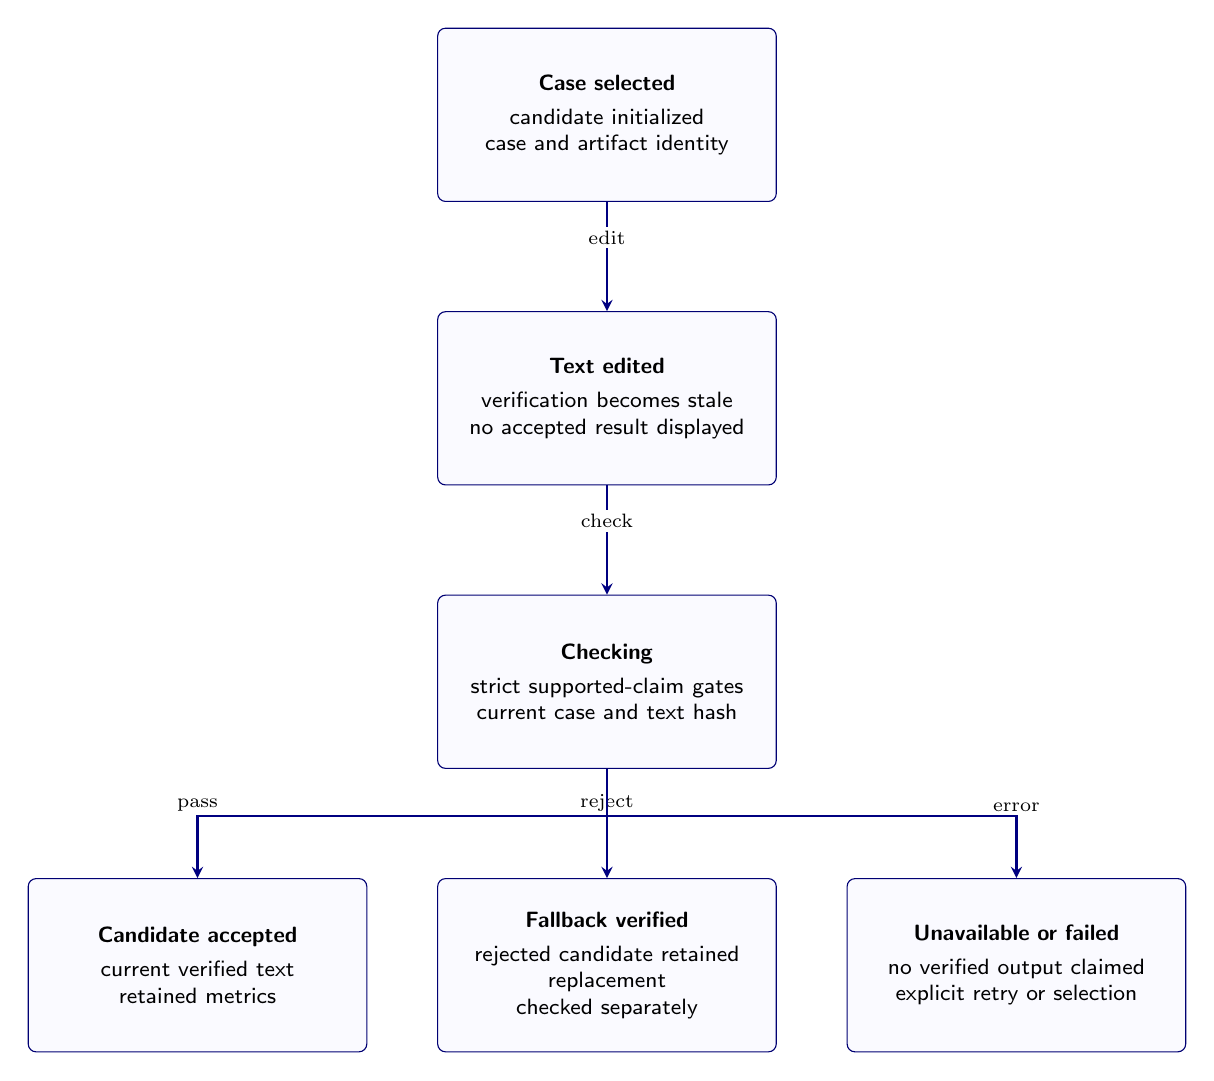
\begin{tikzpicture}[x=1mm,y=1mm,box/.style={draw=blue!45!black,fill=blue!2,rounded corners=1mm,align=center,text width=39mm,minimum height=22mm,inner sep=2mm,font=\sffamily\footnotesize},link/.style={->,>=stealth,draw=blue!50!black,thick}]
\node[box] (selected) at (75,135) {\textbf{Case selected}\\[1mm]candidate initialized\\case and artifact identity};
\node[box] (edited) at (75,99) {\textbf{Text edited}\\[1mm]verification becomes stale\\no accepted result displayed};
\node[box] (checking) at (75,63) {\textbf{Checking}\\[1mm]strict supported-claim gates\\current case and text hash};
\node[box] (accepted) at (23,27) {\textbf{Candidate accepted}\\[1mm]current verified text\\retained metrics};
\node[box] (fallback) at (75,27) {\textbf{Fallback verified}\\[1mm]rejected candidate retained\\replacement checked separately};
\node[box] (error) at (127,27) {\textbf{Unavailable or failed}\\[1mm]no verified output claimed\\explicit retry or selection};
\draw[link] (selected.south) -- ++(0,-6) -| (edited.north) node[pos=.5,above,fill=white,inner sep=.5mm,font=\scriptsize]{edit};
\draw[link] (edited.south) -- ++(0,-6) -| (checking.north) node[pos=.5,above,fill=white,inner sep=.5mm,font=\scriptsize]{check};
\draw[link] (checking.south) -- ++(0,-6) -| (accepted.north) node[pos=.5,above,fill=white,inner sep=.5mm,font=\scriptsize]{pass};
\draw[link] (checking.south) -- ++(0,-6) -| (fallback.north) node[pos=.5,above,fill=white,inner sep=.5mm,font=\scriptsize]{reject};
\draw[link] (checking.south) -- ++(0,-6) -| (error.north) node[pos=.5,above,fill=white,inner sep=.5mm,font=\scriptsize]{error};
\end{tikzpicture}
\caption{Verification state and stale-result invalidation.}\label{fig:state}\end{figure}
\begin{figure}[htbp]\centering\resizebox{\linewidth}{!}{\begin{tikzpicture}[x=1mm,y=1mm,b/.style={draw,text width=135mm,minimum height=23mm,align=center,font=\sffamily\footnotesize},>=Stealth]
\node[b] (ui) at (75,119){\textbf{Presentation}\\Overview / Decision / Evidence / Risk / Explanation / Studies};
\node[b] (app) at (75,81){\textbf{Application}\\Case loading, current-state ownership, confidence policy and emission};
\node[b] (domain) at (75,43){\textbf{Domain}\\Validated records, feature meanings, tolerance/capacity and claim checks};
\node[b] (files) at (75,5){\textbf{Artifacts / runtime}\\Versioned JSON traces, original models, study receipts and local session memory};
\draw[->](ui)--node[right,font=\scriptsize]{user action}(app);\draw[->](app)--node[right,font=\scriptsize]{validated contract}(domain);\draw[->](domain)--node[right,font=\scriptsize]{read / retain identity}(files);
\end{tikzpicture}}
\caption{Current presentation, application, domain and storage layers.}\label{fig:layers}\end{figure}
\begin{figure}[htbp]\centering\resizebox{\linewidth}{!}{\begin{tikzpicture}[x=1mm,y=1mm,b/.style={draw,rounded corners,text width=60mm,minimum height=45mm,align=left,font=\sffamily\footnotesize,inner sep=2mm},>=Stealth]
\node[b] (onboard) at (34,156){\textbf{1. Onboarding}\\Educational purpose / limits\\Data and privacy controls\\Start analysis};
\node[b] (profile) at (116,156){\textbf{2. Profile}\\Capacity + 13 tolerance items\\Binding tier / risk allowance\\Required confidence};
\node[b] (company) at (116,88){\textbf{3. Company selection}\\Audited company universe\\Data-age/coverage status\\Choose horizon};
\node[b] (decision) at (34,88){\textbf{4. Decision and evidence}\\Qualified signal or abstention\\Probability / SHAP / inputs\\Open feature detail};
\node[b] (check) at (34,20){\textbf{5. Explanation/checking}\\User-facing explanation\\Claim report and recovery\\Explicit confidence limitations};
\node[b,dashed] (chat) at (116,20){\textbf{6. Follow-up (planned)}\\Question about current evidence\\Rolling context / citations\\Source-bound verified response};
\draw[->](onboard)--(profile);\draw[->](profile)--(company);\draw[->](company)--(decision);\draw[->](decision)--(check);\draw[->,dashed](check)--(chat);
\node[align=center,font=\scriptsize,text width=143mm] at (75,-23){Wireframes describe the product journey. Dashed follow-up and multi-company/service integrations are future scope; actual screenshots are shown separately.};
\end{tikzpicture}}
\caption{Planned full-product interfaces; not completed software.}\label{fig:final-wireframes}\end{figure}

\chapter{Meeting and Progress Evidence}
Actual meeting dates, participants, supervisor feedback and agreed actions have not been supplied for this increment. No attendance, approval or member contribution is inferred. The team must add authentic records before submission, keeping dates/participants/actions traceable to their original evidence.


\bibliographystyle{IEEEtran}
\bibliography{references/references}
\end{document}

